\chapter*{Wstęp}
\addcontentsline{toc}{chapter}{Wstęp}
W ostatnich latach liczba urządzeń mobilnych na rynku rośnie w bardzo szybkim tempie. Na początku 2017 roku liczba użytkowników urzadzeń mobilnych wynosiła prawie 5 miliardów osób, co stanowi blisko 70\% populacji świata. \cite{Digitali12:online} 

W październiku 2016 roku doszło również do zmiany lidera w zestawieniu udziału poszczególnego rodzaju urządzeń w ruchu internetowym. Pierwszy raz w historii urządzenia mobilne miały większy udział w ruchu internetowym na świecie niż komputery. \cite{Mobilean2:online} 

W Polsce ten udział utrzymuje się na poziomie około 60-65\%. Pod tym kątem należy ona do czołówki państw o największym udziale urządzeń mobilnych w ruchu internetowym. \cite{Desktopv13:online}

Fakt, że Polacy tak chętnie korzystają ze smartfonów i ich funkcjonalności, sprawia że są oni bardzo krytyczni wobec twórców aplikacji mobilnych. Nawet krótka przerwa w działaniu aplikacji (spowodowana na przykład awarią serwera dostarczającego dane), może spowodować pojawienie się wielu krytycznych recenzji. Dlatego zaprojektowanie, zaimplementowanie oraz późniejsze utrzymywanie dobrze ocenianej przez użytkowników aplikacji wymaga wiele wysiłku od autorów aplikacji.

Celem niniejszej pracy jest utworzenie wieloplatformowej aplikacji mobilnej na platformy iOS oraz Android. Wieloplatformowość aplikacji mobilnej jest rozumiana jako możliwość uruchomienia aplikacji na różnych systemach oraz platformach sprzętowych z wykorzystaniem tej samej bazy kodu (ang. \textit{codebase}).

Aspekt wieloplatformowości aplikacji nie jest nowym tematem. Pierwszym krokiem ku aplikacjom wieloplatformowym było powstanie języka programowania Java w połowie lat dziewięćdziesiątych XX wieku. Dzięki temu, że kod źródłowy programów tworzonych w Javie kompiluje się do kodu pośredniego, który potem jest wykonywany przez wirtualną maszynę Javy (ang. \textit{Java Virtual Machine}), takie aplikacje działają niezależnie od platformy. Jedynym warunkiem jest działająca wirtualna maszyna Javy dla danej platformy. Główną wadą takiego rozwiązania jest słabsza wydajność niż w przypadku aplikacji, których kod jest kompilowany do kodu maszynowego. 
\newpage
Kolejnym kamieniem milowym w dziedzinie wieloplatformowości było pojawienie się pierwszych smartfonów na rynku. Premiera pierwszej wersji iPhone'a zaprojektowanego przez Apple, kupienie przez Google Androida w 2007 roku oraz uruchomienie scentralizowanych sklepów z aplikacjami rok później, zredefiniowało rynek aplikacji. Obok aplikacji webowych oraz desktopowych pojawił się trzeci gracz - aplikacje mobilne. 

To właśnie zadomowienie się na rynku tych dwóch platform (Android oraz iOS) sprawiło, że znowu głośno zaczęto mówić o tym jak tworząc jedną aplikacje zapewnić jej działanie na obu platformach. W 2011 roku pojawił się w tej dziedzinie przełom. W tym czasie upowszechniły się dwa frameworki do tworzenia aplikacji wieloplatformowych. 

Pierwszym z nich jest PhoneGap (obecnie Apache Cordova). Jest to framework stworzony przez firmę Nitobi, kupiony przez firmę Adobe w 2011 roku. PhoneGap umożliwia tworzenie aplikacji wieloplatformowych w oparciu o najnowsze standardy webowe takie jak HTML5, CSS3 oraz JavaScript. Dzięki wbudowanej obsłudze standardu HTML5 w obu systemach, można tworzyć aplikacje wykorzystujące większość czujników dostępnych w urządzeniu (między innymi odbiornik GPS oraz akcelerometr). Minusem tego rozwiązania są ograniczenia w kontekście doświadczenia użytkownika (ang. \textit{user experience}). Aplikacja utworzona z wykorzystaniem PhoneGap'a nie zapewnia wszystkich, specyficznych dla danej platformy, zachowań interfejsu w porównaniu z aplikacjami natywnymi. Obecnie istnieje wiele frameworków opartych o PhoneGap'a, takich jak na przykład Ionic Framework (wykorzystujący Angulara), jednak wszystkie borykają się z podobnymi problemami.

Drugim jest Xamarin. Stworzony przez firmę o takiej samej firmie, framework umożliwia tworzenie w pełni natywnych aplikacji na Androida oraz iOS'a z wykorzystaniem kodu źródłowego w języku C\#. Właśnie ze względu na natywność tworzonych aplikacji, Xamarin został wybrany do realizacji projektu. Więcej informacji o Xamarin'ie znajduje się w podrozdziałach \ref{sec:xamAnd} oraz \ref{sec:xamiOS}.

Niniejsza praca składa się z 6 rozdziałów. W pierwszym rozdziale znajduje się wprowadzenie do problematyki tworzenia systemów rezerwacji biletów łącznie z przeglądem istniejących rozwiązań na rynku. Drugi rozdział jest poświęcony opisowi głównych technologii oraz narzędzi deweloperskich wykorzystanych w trakcie realizacji projektu. W trzecim rozdziale znajduje się opis wstępnych założeń projektowych. Czwarty rozdział zawiera szczegółowy projekt aplikacji. W piątym rozdziale znajdują się najważniejsze aspekty oraz problemy fazy implementacji. Szósty rozdział jest poświęcony podsumowaniu realizacji projektu.

\chapter{Wprowadzenie do problematyki}
Systemy rezerwacyjne są to jedne z najczęściej spotykanych systemów we współczesnym świecie. Są one stosowane w wielu branżach. Poczynając od branży hotelarskiej, przez branżę lotniczą kończąc na branży rozrywkowej. Postęp technologiczny, który obserwujemy od początku XXI wieku, pozwolił na zwiększenie skali prowadzonego biznesu. Elektroniczne systemy rezerwacji biletów pozwoliły m.in. na powstanie sieci kin składające się z multipleksów, które są obecnie tak chętnie oblegane przez widzów. Dzięki nim udało się, pomimo dużej skali wzrostu, uniknąć chaosu organizacyjnego oraz znacząco zwiększyć przychody, które pozwoliły na zwrot poniesionych inwestycji. 

Dzisiaj nie wyobrażamy sobie stania w kolejce po papierowy bilet na interesujący nas seans. Większość ludzi posiada komputer czy też smartphone'a i za pomocą kilku kliknięć dokonują zakupu biletu. Taki bilet okazują potem w formie elektronicznej na ekranie smartphone'a lub papierowej - wydrukowany na domowej drukarce.

\subsection*{Obecne rozwiązania na rynku}
W związku ze stopniem skomplikowania takiego systemu, ilością potencjalnych użytkowników oraz gromadzonych danych, sztuką jest stworzenie systemu, który będzie jednocześnie wydajny, bezpieczny i przyjazny użytkownikowi. 

W Polsce swoje usługi oferuje blisko 500 kin, z czego blisko 13\% stanowią multipleksy, które realizują ponad 50\% wszystkich seansów. Większość multipleksów jest obsługiwana przez kilku operatorów kinowych, tworząc w ten sposób sieci kin.\cite{Cinema:1}

Wszyscy główni gracze na rynku posiadają dedykowane systemy rezerwacji w wersji webowej. Gorzej wygląda to jeśli chodzi o dedykowane aplikacje dla urządzeń mobilnych z systemami Android oraz iOS, gdzie tylko dwóch operatorów zadbało o przygotowanie odpowiednich aplikacji.

\subsubsection*{Kino Helios}
Aplikacja dla platform Android oraz iOS  pozwalająca na rezerwację oraz zakup biletów kin Helios. Umożliwia szybkie przeglądanie repertuaru, oglądanie zwiastunów filmów oraz dostarcza informacje o zapowiedziach kinowych. Jej główną cechą jest integracja z systemem płatności SkyCash \cite{Skycash:online}, co wymaga utworzenia konta na wyżej wspomnianej platformie w celu dokonania zakupu lub rezerwacji biletów. 

\begin{figure}[h]
\centering
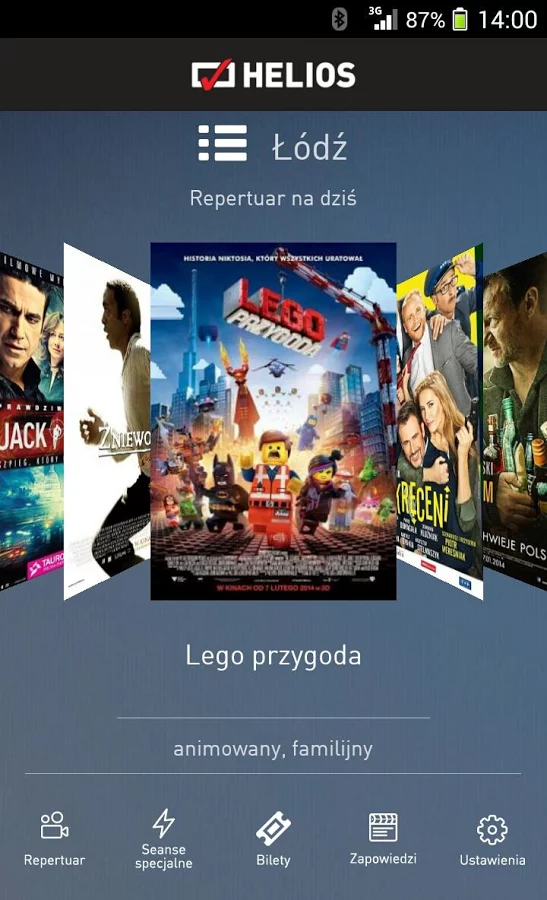
\includegraphics[width=0.5\textwidth]{img5}
\caption{Główny ekran aplikacji "Kino Helios"}
\end{figure}

\begin{figure}[h]
\centering
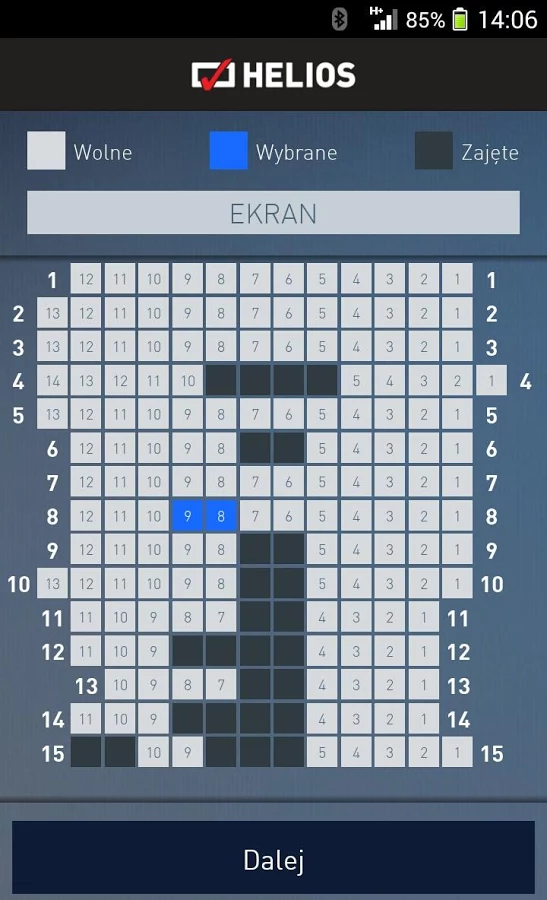
\includegraphics[width=0.5\textwidth]{img6}
\caption{Ekran wyboru miejsca na sali - aplikacja "Kino Helios"}
\end{figure}

Charakteryzuje się dość prostym i intuicyjnym interfejsem - podobnym na obu platformach. Aplikacja jest dostępna za darmo w sklepach z aplikacjami: Google Play Store  \cite{KinoHeli13:online} oraz Apple App Store \cite{Aplikacj38:online}. Obie wersje są średnio oceniane przez użytkowników na około 4 w skali 5 stopniowej, jednak z licznymi zastrzeżeniami zawartymi w recenzjach, głównie dotyczącymi wsparcia dla nowych wersji systemu. Jako, że aplikacja jest zbudowana we współpracy z firmą Skycash, rzadko kiedy sugestie użytkowników, mają odzwierciedlenie w usprawnieniach w aplikacji.
\newpage
\subsubsection*{Multikino}
Aplikacja dla platform Android oraz iOS pozwalająca na rezerwację oraz zakup biletów kin sieci Multikino. Jej interfejs oraz funkcjonalność jest praktycznie identyczna jak w aplikacji "Kino Helios" wspomnianej wcześniej. Podobnie jak w wyżej wymienionej aplikacji, wymagane jest utworzone konto w systemie płatności SkyCash.

\begin{figure}[h]
\centering
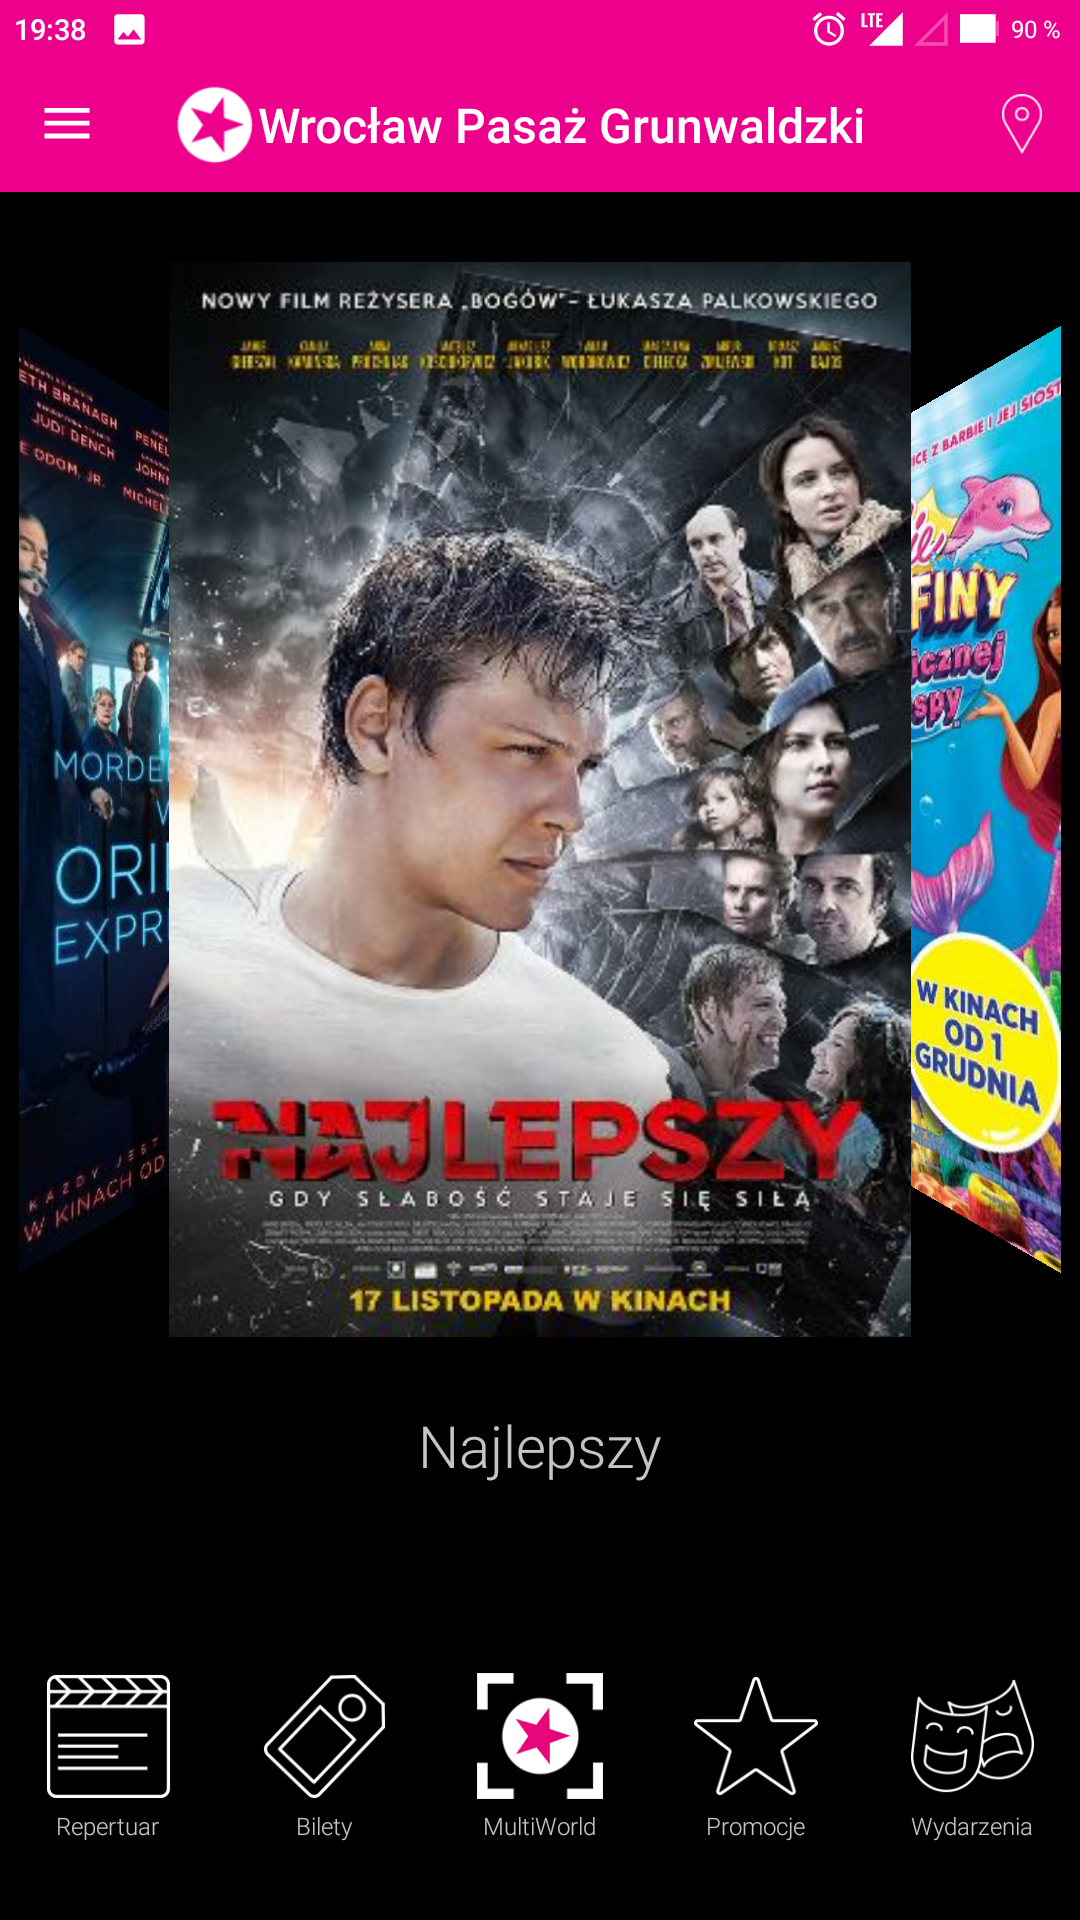
\includegraphics[width=0.5\textwidth]{img7}
\caption{Główny ekran aplikacji "Multikino"}
\end{figure}

\newpage
Interfejs aplikacji jest co do zasady identyczny jak w aplikacji "Kino Helios". Aplikacja jest dostępna za darmo w sklepach z aplikacjami: Google Play Store \cite{Multikin60:online} oraz Apple App Store \cite{Aplikacj40:online}. Obie wersje są średnio oceniane przez użytkowników na około 4 w skali 5 stopniowej, z wieloma krytycznymi opiniami w recenzjach. Podobnie jak w przypadku poprzedniej aplikacji, sugestie użytkowników nie mają wpływu na zmiany w aplikacji.
\chapter{Technologie i narzędzia wykorzystywane w pracy}
W każdym projekcie sytemu informatycznego bardzo ważny jest dobór odpowiednich technologii i narzędzi do rodzaju projektu. W poniższym rozdziale zostały opisane wybrane technologie oraz narzędzia deweloperskie, wspomagające zapewnienie jakości kodu, wykorzystywane w trakcie implementacji systemu.
\section{Xamarin.Android}
\label{sec:xamAnd}
Xamarin.Android jest to platforma programistyczna, stworzona w oparciu o \textit{.NET Framework}, do tworzenia aplikacji na system operacyjny Android z wykorzystaniem natywnych metod SDK (\textit{Software Development Kit}) systemu Android. Z pomocą wyżej wymienionej platformy, aplikacje są tworzone w języku C\# , co w połączeniu z implementacją Xamarin.Android, daje możliwość wykorzystywania specyficznych cech języka takich jak np. \textit{LINQ}. \cite{RefWorks:4}

Kod źródłowy w C\#, w celu uzyskania natywnej aplikacji, jest kompilowany do IL (\textit{Common Intermediate Language}) z wykorzystaniem kompilatora MonoVM. MonoVM jest kompilatorem typu JIT (\textit{just-in-time compiler}). Program jest kompilowany w trakcie wykonywania, przed wykonaniem  danego fragmentu kodu, do kodu maszynowego.
Niewykorzystane klasy zawarte w frameworku są podczas kompilowania aplikacji usuwane z wykorzystaniem \textit{linkera}, w celu zmniejszenia rozmiaru aplikacji.\cite{RefWorks:3} \cite{Part1–Un34:online} \cite{Linkingo58:online} 

Aplikacja działa obok natywnych aplikacji (napisanych w językach Java lub Kotlin) w ART (\textit{Android Runtime} - środowisko uruchomieniowe systemu Android). Interakcje z wykorzystaniem natywnych typów odbywają się z pomocą JNI (\textit{Java Native Interface}) \cite{Part1–Un34:online}

\section{Xamarin.iOS}
\label{sec:xamiOS}
Xamarin.iOS, podobnie jak wspomniany w poprzednim podrozdziale Xamarin.Android, jest to platforma programistyczna, stworzona w oparciu o .NET Framework, do tworzenia aplikacji na system operacyjny iOS. Wykorzystuje ona natywne metody SDK (\textit{Software Development Kit}) systemu iOS. Aplikacje są tworzone z wykorzystaniem języka C\#.

Kod źródłowy jest kompilowany z użyciem kompilacji AOT (\textit{Ahead-Of-Time}) do języka assemblera dla procesorów ARM. Do kodu jest dołączony framework .NET, którego nieużywane klasy są usuwane przy pomocy \textit{linkera} w celu zmniejszenia rozmiaru aplikacji.\cite{RefWorks:4} \cite{Part1–Un34:online} \cite{Linkingo42:online}

Jako, że firma Apple - twórca systemu iOS, nie pozwala na dynamiczne generowanie kodu w trakcie wykonywania programu, niektóre cechy języka C\# nie są dostępne dla twórcy aplikacji. (ograniczenia głównie dotyczą klas generycznych \cite{Limitati57:online} oraz mechanizmu refleksji \cite{Limitati74:online})
\section{ASP.NET Core}
\label{sec:aspCore}
ASP.NET Core jest to wieloplatformowy, otwarty framework, stworzony przez firmę Microsoft, służący do budowania nowoczesnych aplikacji internetowych. Umożliwia on między innymi budowanie aplikacji oraz serwisów internetowych czy też aplikacji działąjących na urządzeniach IoT \textit{Internet of Things}.\cite{RefWorks:8}

Z racji wieloplatformowości, aplikacje mogą być tworzone oraz uruchamiane na systemach z rodziny Windows, Linux oraz macOS. Jako środowisko uruchomieniowe wykorzystywany jest .NET Framework (Windows) lub .NET Core (Windows/Linux/macOS) \cite{RefWorks:9}\cite{Introduc95:online}
 

\section{Entity Framework Core}
\label{sec:entityCore}
Entity Framework (EF) Core jest to wieloplatformowy ORM (\textit{Object-Relational Mapper} - mapper obiektowo-relacyjny) zbudowany przez firmę Microsoft w oparciu o .NET Core, umożliwiający pracę z relacyjną bazą danych z wykorzystaniem natywnych obiektów ze środowiska .NET.

EF Core prawie całkowicie eliminuje konieczność tworzenia ręcznie zapytań SQL do bazy danych. Można z niego korzystać z wieloma silnikami bazodanowymi np. \textit{Microsoft SQL Server}, \textit{Oracle}.

Z wykorzystaniem EF Core, dostęp do danych odbywa się za pośrednictwem modelu. Model składa się z klas opisujących modele związków encji oraz kontekstu, który reprezentuje sesję połączenia z bazą danych, umożliwiając tworzenie zapytań oraz zapisywanie danych.

EF Core umożliwia wygenerowanie modelu na podstawie istniejącej bazy danych (podejście \textit{Database-First}) lub wygenerowanie bazy danych na podstawie przygotowanego modelu z wykorzystaniem mechanizmu migracji (podejście \textit{Code-First})\cite{QuickOve99:online}

\section{Dapper}
\label{sec:dapper}
Dapper jest to otwarty (\textit{open-source}) ORM (\textit{Object-Relational Mapper} - mapper obiektowo-relacyjny). Określa się go czasami również jako microORM, ze względu na brak wszystkich funkcjonalności charakteryzujących klasyczne ORM-y takie jak np. opisany w poprzednim podrozdziale Entity Framework Core [\ref{sec:entityCore}]. 

Zaletą Dapper-a jest znacznie mniejszy narzut wydajnościowy, co można zauważyć przy odczycie danych. W porównaniu z Entity Framework, Dapper przy odczycie danych potrafi być ponad 10 razy szybszy (dane dla 500 operacji SELECT).

Od strony technicznej Dapper jako biblioteką rozszerzającą interfejs \textit{IDbConnection} dostępny w ramach .NET Framework. Dzięki takiej implementacji, Dapper zapewnia podobną wydajność jak ręczne mapowanie danych z wykorzystaniem klasy \textit{SqlDataReader} \cite{StackExc69:online}  
\section{MVVMCross}
\label{sec:mvvmCross}
MVVMCross jest to otwarty (\textit{open-source}) framework wspomagający tworzenie aplikacji według wzorca architektonicznego Model-View-ViewModel. MVVMCross jest przygotowany specjalnie pod kątem platformy Xamarin. Wspiera tworzenie aplikacji w technologiach Xamarin.Android, Xamarin.iOS, Xamarin Forms, Universal Windows Platform (UWP) oraz Windows Presentation Framework (WPF).

Do głównych funkcjonalności MVVMCross należą: wsparcie dla wzorca MVVM, system nawigacji, \textit{data binding}, wsparcie dla specyficznych dla danej platformy funkcji, wbudowany system wstrzykiwania zależności \textit{Dependency Injection} oraz odwracania kontroli \textit{Inversion of Control}, system pluginów dla najczęściej wykorzystywanych funkcji oraz wsparcie dla testów jednostkowych. \cite{GettingS94:online}

Dzięki wykorzystaniu MVVM Cross, można współdzielić nawet do 90\% kodu pomiędzy aplikacjami na różne platformy.
\newpage
\section{Identity Server 4}
\label{sec:is4}
Identity Server 4 jest to otwarty (ang. \textit{open-source}) framework dodający obsługę OpenID Connect oraz OAuth 2.0 dla aplikacji stworzonych w ASP.NET Core. Framework jest udostępniany jako biblioteka do pobrania z repozytorium paczek NuGet. Z jego pomocą uzyskujemy następujące funkcjonalności:
\begin{itemize}
\item {Scentralizowana logika logowania do aplikacji}
\item {Możliwość pojedynczego logowania \textit{single sign-on}}
\item {Zabezpieczenie WebAPI z wykorzystaniem tokenów dostępu \textit{access token}}
\item {Możliwość logowania z pomocą zewnętrznych dostawców tożsamości takich jak Facebook, Google}
\end{itemize}
\section{Team Foundation Server}
\label{sec:team}
Team Foundation Server jest to system firmy Microsoft wspierający zarządzanie projektem informatycznym przez cały cykl życia oprogramowania.
Do jego funkcjonalności zaliczamy:
\begin{itemize}
\item system kontroli wersji/repozytorium kodu (do wyboru Git lub Team Foundation Version Control)\cite{Kontrola99:online},
\item wsparcie przy planowaniu prac w zespołach projektowych w zespołach korystających z metodyk zwinnych (Agile/Scrum) oraz modelu kaskadowego (\textit{waterfall})\cite{Narzedzi82:online},
\item \textit{DevOps} - automatyzacja procesu wytwarzania oprogramowania w celu zapewnienia jakości - automatyczne budowanie aplikacji, uruchamianie testów, dostarczanie metryk dotyczących kodu (np. \textit{Code Coverage} - pokrycie kodu testami lub ocena długu technologicznego), automatyczne wdrażanie aplikacji, wsparcie dla wielu środowisk wdrożeniowych, system zarządzania wydaniami\cite{Ciaglain95:online}
\item wsparcie dla wielu języków programowania oraz obsługa serwerów budujących z systemami Windows, Linux oraz macOS \cite{Buildand77:online}
\item Integracja z zewnętrznymi narzędziami: np. środowiskami programistycznymi (takimi jak np. Visual Studio lub Eclipse), platformami typu Visual Studio Mobile Center (więcej w podrozdziale \ref{sec:hockeyapp})
\end{itemize}
\section{Microsoft Azure}
\label{sec:azure}
Microsoft Azure jest to usługa chmury obliczeniowej stworzona przez firmę Microsoft, służąca do tworzenia, testowania, wdrażania i zarządzania aplikacji oraz serwisów znajdujących się w centrach danych firmy Microsoft.

Microsoft Azure udostępnia usługi w modelach IaaS (\textit{Infrastructure as a Service}), PaaS (\textit{Platform as a Service}) oraz SaaS (\textit{Service as a Service}). Wspiera różne języki programowania, narzędzia oraz frameworki, zarówno stworzone przez Microsoft jak i firm trzecich. 

Do najpopularniejszych usług należą między innymi:
\begin{itemize}
\item maszyny wirtualne (IaaS) pozwalające na uruchomienie obrazów systemów Windows oraz Linux
\item \textit{App Service} udostępniany jako usługa w modelu PaaS umożliwia hostowanie aplikacji internetowych oraz mobilnych stworzonych w różnych technologiach. Umożliwia integrację z instancją Team Foundation Server (podrozdział \ref{sec:team}) w ramach ciągłej integracji oraz ciągłego wdrażania.
\item baza danych SQL działająca w technologii Microsoft SQL Server.
\end{itemize}
\section{Visual Studio Mobile Center}
\label{sec:hockeyapp}
Visual Studio Mobile Center jest to platforma deweloperska działająca w chmurze stworzona przez firmę Microsoft. Do głównych usług oferowanych należą:
\begin{itemize}
\item po podpięciu repozytorium kodu z usługi Team Foundation Server - możliwość budowania aplikacji mobilnych,
\item możliwość testowania aplikacji na podstawie testów interfejsu przygotowanych z wykorzystaniem różnych framework'ów (np. Xamarin UI Tests)
\item możliwość dystrybucji aplikacji wśród zamkniętej grupy użytkowników (umożliwia prowadzenie zamkniętych testów aplikacji)
\item gromadzenie informacji o błędach aplikacji
\item gromadzenie statystyk użycia aplikacji - informacje o zachowaniach użytkowników, urządzeniach na których działa aplikacja, zdarzeniach w trakcie działania aplikacji
\end{itemize}
\chapter{Założenia projektowe}
\label{zal}
W tym rozdziale zostaną omówione założenia projektowe systemu. Pierwszy podrozdział jest poświęcony opisowi przedmiotu pracy. W podrozdziałach drugim oraz trzecim zostały opisane wymagania (odpowiednio funkcjonalne i niefunkcjonalne) na system. Ostatni podrozdział jest to opis zaprojektowanej architektury systemu.
\section{Przedmiot pracy}
Przedmiotem pracy jest utworzenie aplikacji mobilnej na platformy Android oraz iOS, umożliwiającej rezerwację i zakup biletów kinowych w ramach sieci kin, wraz z towarzyszącą aplikacją serwerową. Aplikacja kliencka będzie utworzona w oparciu o platformę Xamarin [\ref{sec:xamAnd}][\ref{sec:xamiOS}], natomiast aplikacja serwerowa w oparciu o framework ASP.NET Core [\ref{sec:aspCore}]
\section{Wymagania funkcjonalne}
\label{sec:func}
System powinien spełniać następujące wymagania funkcjonalne. Przy definiowaniu wymagań przyjęto następujących aktorów - Klient, Pracownik kina, Administrator systemu, System 
\begin{enumerate}
\item Jako Klient, chcę mieć możliwość stworzenia konta użytkownika na podstawie adresu e-mail, w celu zachowania preferencji użytkownika pomiędzy urządzeniami.
\item Jako Klient, chcę mieć możliwość stworzenia konta użytkownika z wykorzystaniem konta w jednym ze wspieranych portali społecznościowych (Facebook, Twitter, Google), w celu przyspieszenia procesu tworzenia konta.
\item Jako Klient, chcę mieć możliwość modyfikacji informacji o koncie użytkownika, w celu wygodnej aktualizacji danych.
\item Jako Klient, chcę mieć możliwość zresetowania hasła do konta użytkownika, w celu odzyskania dostępu do konta. 
\item Jako Klient, chcę mieć możliwość wyboru domyślnego kina, w celu łatwiejszego dostępu do aktualnego repertuaru.
\item Jako Klient, chcę mieć możliwość przeglądania aktualnego repertuaru w danym kinie, w celu zapoznania się z ofertą kina.
\item Jako Klient, chcę mieć możliwość przeglądania podstawowych informacji o filmie z repertuaru, w celu zapoznania się z krótkim opisem filmu. 
\item Jako Klient, chcę mieć możliwość złożenia rezerwacji biletu(ów) na wybrany seans w wybranym kinie, w celu późniejszej finalizacji zamówienia przed seansem.
\item System anuluje wszystkie niepotwierdzone rezerwacje 30 minut przed planowanym początkiem seansu. 
\item Jako Klient, chcę mieć możliwość zakupu biletu(ów) na wybrany seans w wybranym kinie, w celu braku konieczności kupna biletu w kasie stacjonarnej przed seansem.
\item Jako Klient, chcę mieć możliwość dokonania zapłaty za zakupione bilety za pośrednictwem zewnętrznego systemu płatności elektronicznych, w celu szybszej finalizacji zamówienia
\item Jako Klient, chcę mieć możliwość zwrotu zakupionych biletów do 3 godzin przed planowanym seansem, w celu odzyskania pieniędzy za niewykorzystane bilety.
\item Jako Klient, chcę mieć możliwość wyboru miejsc na podstawie widoku sali kinowej, w celu świadomego wyboru miejsca na sali kinowej.
\item Jako Klient, chcę mieć możliwość wyboru rodzaju biletu przy wyborze miejsc, w celu wyboru odpowiedniego rodzaju biletu (np. ulgowego dla osoby niepełnoletniej).
\item Jako Klient, chcę mieć możliwość przeglądania historii rezerwacji oraz zakupionych biletów, w celu   zapoznania się z poprzednimi transakcjami.
\item Jako Klient, chcę mieć możliwość okazania biletu w formacie kodu QR, w celu ułatwienia weryfikacji biletu przy wejściu na salę kinową.
\item Jako Klient, chcę mieć możliwość okazania biletu pomimo braku połączenia z siecią Internet, w celu ograniczenia powszechnych problemów dotyczących połączenia internetowego przy okazywaniu biletu.\newline
\item Jako Pracownik kina, chcę mieć możliwość modyfikacji podstawowych danych o kinie, w celu aktualizacji danych.
\item Jako Pracownik kina, chcę mieć możliwość modyfikacji informacji o salach dostępnych w kinie, w celu aktualizacji ilości dostępnych miejsc na sali kinowej.
\item Jako Pracownik kina, chcę mieć możliwość modyfikacji repertuaru kina, w celu aktualizacji oferty kina.
\item Jako Pracownik kina, chcę mieć możliwość potwierdzenia rezerwacji klienta, w celu finalizacji zamówienia.
\item Jako Pracownik kina, chcę mieć możliwość anulowania rezerwacji klienta, w celu zapewnienia większego wyboru miejsc dla pozostałych Klientów.
\item Jako Pracownik kina, chcę mieć możliwość dokonania sprzedaży biletów klientom w kasie biletowej, w celu umożliwienia kupna biletów przez Klientów nie posiadających aplikacji.
\item Jako Administrator systemu, chcę mieć możliwość dodawania, modyfikowania i usuwania informacji o kinach należących do sieci kin, w celu weryfikacji danych o kinach.
\item Jako Administrator systemu, chcę mieć możliwość tworzenia oraz modyfikacji kont użytkowników oraz przydzielania im ról, w celu zarządzania dostępu użytkowników do systemu.
\end{enumerate}
Powyższa lista jest pełnym zbiorem wymagań, które powinny się znaleźć w ostatecznej wersji systemu. Prototyp systemu, będący celem pracy, będzie miał zaimplementowane wszystkie funkcjonalności dotyczące roli Klienta tj. wymagania od pierwszego do siedemnastego.
\newpage
\section{Wymagania niefunkcjonalne}
Zbiór tych wymagań definiuje, jakie wymagania na system mają zostać spełnione, oprócz wymagań funkcjonalnych. Wymagania te głównie dotyczą wydajności, bezpieczeństwa i tym podobnych aspektów.
\begin{enumerate}
\item System powinien być dostępny bez przerwy. (Dostępność na poziomie 99,9\%)
\item System jest w stanie obsługiwać wiele jednocześnie podłączonych urządzeń.
\item Do poprawnego korzystania ze wszystkich funkcji oferowanych przez aplikację, wymagane jest stałe połączenie internetowe.
\item W celu zapewnienia odpowiedniego poziomu bezpieczeństwa, połączenie między serwerem i klientem ma być szyfrowane.
\item System ma wspierać również mechanizm sesji, jako dodatkowy mechanizm zabezpieczający połączenie.
\item Aplikacja kliencka powinna być dostępna na systemach Android (w wersji 4.4 i wyższej) oraz iOS (w wersji 8.0 i wyższej).
\item Aplikacja kliencka powinna zostać uruchomiona na urządzeniu mobilnym niezależnie od stanu połączenia internetowego.
\item Aplikacja serwerowa powinna móc być uruchomiona na serwerach z systemami rodziny Windows Server (wersja 2012 R2 i wyżej)

\end{enumerate}
\newpage
\section{Opis podstawowej architektury systemu}
\subsection*{Architektura logiczna}
System będzie składał się z czterech aplikacji. 

\par Pierwszą z nich jest aplikacja serwerowa, realizowana w architekturze trójwarstwowej (podział na warstwę prezentacji, logiki biznesowej oraz dostępu do danych). Dzięki takiemu podziałowi, w którym wyższa warstwa nie wie o logice zawartej w niższej warstwie (\textit{black box}) zapewniamy m.in. dużą skalowalność rozwiązania (każdą warstwę możemy skalować według potrzeb) oraz ułatwione testowanie rozwiązania poprzez brak skomplikowanych zależności pomiędzy warstwami.

\par Operacje na bazie danych aplikacji będą wykonywane w warstwie dostępu do danych z częściowym wykorzystaniem podejścia CQRS (\textit{Command Query Responsibility Segregation}), które zapewni jeszcze lepszą skalowalność rozwiązania poprzez, przede wszystkim oddzielenie operacji zapisu danych od ich odczytu. Więcej szczegółów na temat podejścia CQRS oraz jego implementacji znajduje się w podrozdziale~\ref{sec:cqrs}

\par Druga aplikacja jest to aplikacja serwerowa, służąca do autentykacji i autoryzacji użytkowników. Wykorzystuje ona framework Identity Server (więcej w podrozdziale \ref{sec:is4}), który pozwala na łatwe utworzenie aplikacji będącej dostarczycielem tożsamości (ang. \textit{identity provider})

\par Pozostałą część systemu stanowią aplikacje mobilne działająca pod kontrolą systemu Android oraz iOS. Aplikacje te będą implementowane z wykorzystaniem platformy Xamarin. Dzięki temu możemy mówić o aplikacji wieloplatformowej, ponieważ większość kodu aplikacji (głównie chodzi tutaj o logikę zawartą w aplikacji) jest współdzielona. Aby umożliwić współdzielenie kodu, będzie zastosowany wzorzec architektoniczny Model-View-ViewModel. Dzięki temu wzorcowi dokonujemy separacji aplikacji na warstwy: widoku (View), logiki interfejsu (ViewModel) oraz modelu danych. Logika interfejsu oraz modelu danych są współdzielone, natomiast osobne widoki odpowiadają specyfice poszczególnych systemów. Wyseparowane warstwy sprawiają, że kod aplikacji jest o wiele bardziej testowalny oraz łatwiejszy w utrzymaniu. Do przechowywania danych lokalnych aplikacji posłuży baza danych SQLite.
\newpage
\subsection*{Architektura fizyczna}
\label{fizy}
Aplikacje serwerowe zbudowane będą w oparciu o framework ASP.NET Core. Będzie mieć ona możliwość pracowania na serwerach z systemami rodziny Windows Server. Wykorzystywany serwer WWW to IIS (\textit{Internet Information Services}) lub Apache.

\par Aplikacje serwerowe będą komunikować się z silnikiem bazodanowym Microsoft SQL Server znajdującym się na osobnych serwerach (działającym pod kontrolą dystrybucji systemu Windows Server lub Linux), z wykorzystaniem protokołu TLS/SSL w celu zapewnienia odpowiedniego poziomu bezpieczeństwa.

\par W ramach realizowanego prototypu, serwery aplikacji oraz bazy danych będą hostowane na platformie obliczeniowej Microsoft Azure. 

\par Aplikacje klienckie działające na urządzeniach z systemami Android oraz iOS, będą komunikowały się z serwerem aplikacji, wykorzystując udostępnione przez aplikację \textit{RESTful API} po uprzedniej autoryzacji przez serwis autoryzaujący. Formatem przesyłanych danych jest \textit{JSON}. Komunikacja odbywa się za pośrednictwem protokołu HTTPS (ruch jest szyfrowany).
\begin{figure}[h]
\centering
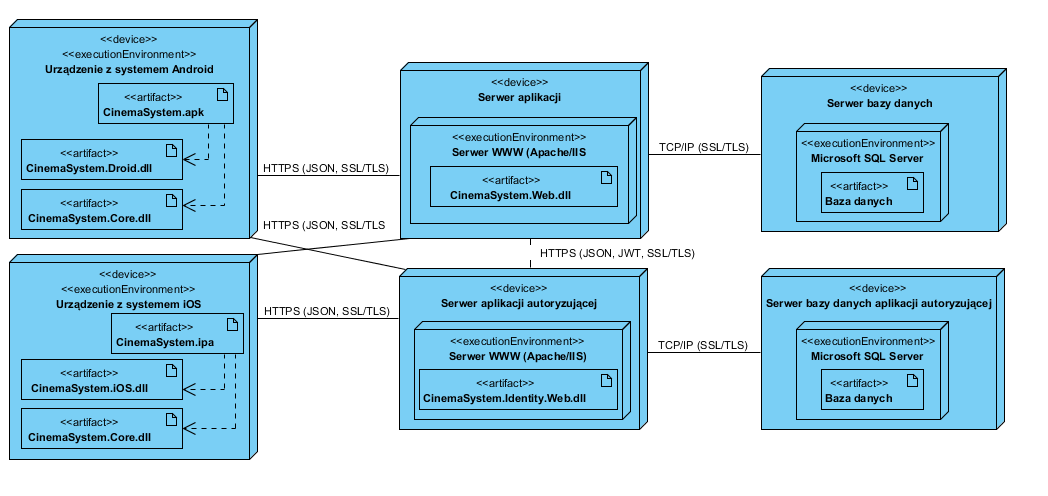
\includegraphics[width=1\textwidth]{img1}
\caption{Architektura fizyczna systemu}
\end{figure}
\chapter{Projekt aplikacji}
Dobrze przygotowany projekt aplikacji jest kluczowy w przygotowaniu aplikacji mobilnej mającej w przyszłości zadowolić zleceniodawcę, udziałowców oraz użytkownika końcowego. W pierwszym podrozdziale zostały opisane przypadki użycia aplikacji w postaci uproszczonych scenariuszy. Drugi podrozdział zawiera przygotowane szkice interfejsu (mockup'y) wraz z opisem. Ostatni podrozdział jest poświęcony diagramom klas poszczególnych części systemu wraz z opisem.
\section{Przypadki użycia}
Wymienione poniżej przypadki użycia powstały na podstawie historyjek użytkownika wymienionych w podrozdziale \ref{sec:func} wybranych do realizacji w ramach prototypu aplikacji.
\par
\begin{tabularx}{\textwidth}{|l|X|}
\hline
1                      & Rejestracja                                                                                                                                                                                                                                                                                                                                                                                                                                   \\ \hline
Aktor                  & Klient, System \\ \hline
Warunki początkowe     & Klient nie jest zalogowany                                                                                                                                                                                                                                                                                                                                                                                                                    \\ \hline
Zdarzenie inicjujące   & Klient wyraża chęć rejestracji konta                                                                                                                                                                                                                                                                                                                                                                                                          \\ \hline
Przebieg w krokach     & 1. System wyświetla formularz rejestracji zawierające pole do wpisania adresu e-mail oraz dwa pola do wpisania hasła \newline 2. Klient wypełnia formularz rejestracji \newline 3. System weryfikuje poprawność danych, tworzy konto oraz wysyła maila z powiadomieniem o pomyślnej rejestracji z linkiem aktywującym konto. \newline 4. Klient przechodzi pod adres zawarty w wiadomości email \newline 5. System aktywuje konto \\ \hline
Przebiegi alternatywne & a)  1. System pokazuje formularz logowania. \newline 2. Klient wybiera opcję ``Zaloguj za pomocą Facebook`` \newline 3. System przekierowuje do portalu Facebook \newline 4. Klient się loguje na swoje konto Facebook oraz wyraża zgodę na użycie danych przez System. \newline 5. System tworzy aktywne konto oraz wysyła maila z powiadomieniem o pomyślnej rejestracji \\ \hline
Sytuacje wyjątkowe     &System wykrywa konto o takim samym adresie e-mail i wyświetla odpowiedni komunikat o błędzie. \newline System wykrywa hasło niespełniające polityki tworzenia haseł i wyświetla odpowiedni komunikat o błędzie. \\ \hline
Warunki końcowe        &                                                                                                                                                                                                                                                                                                                                                                                                                                          System tworzy aktywowane konto dla Klienta. \\ \hline
\end{tabularx}
\newpage
\begin{tabularx}{\textwidth}{|l|X|}
\hline
2                      & Logowanie                                                                                                                                                                                                                                                                                            \\ \hline
Aktor                  & Klient, System \\ \hline
Warunki początkowe     & Klient nie jest zalogowany                                                                                                                                                                                                                                                                           \\ \hline
Zdarzenie inicjujące   & Klient wyraża chęć zalogowania się na konto                                                                                                                                                                                                                                                          \\ \hline
Przebieg w krokach     & 1. System wyświetla formularz logowania, który zawiera pole na adres e-mail oraz hasło.\newline 2. Klient wypełnia formularz.\newline 3. System weryfikuje formularz. \\ \hline
Przebiegi alternatywne &  1. System pokazuje formularz logowania.\newline 2. Klient wybiera opcję "Zaloguj za pomocą Facebook"\newline 3. System przekierowuje do portalu Facebook\newline 4. Klient się loguje na swoje konto Facebook.\newline 5. System weryfikuje dane otrzymane od portalu Facebook \\ \hline
Sytuacje wyjątkowe     & System nie wykrywa konta o podanym adresie e-mail i wyświetla odpowiedni komunikat o błędzie.\newline System wykrywa, że podane hasło nie pasuje do podanego konta i wyświetla odpowiedni komunikat o błędzie \\ \hline
Warunki końcowe        & Klient zostaje zalogowany.                                                                                                                                                                                                                                                                           \\ \hline
\end{tabularx}
\par
\begin{tabularx}{\textwidth}{|l|X|}
\hline
3                      & Resetowanie hasła                                                                                                                                                                                                                                                                                                                                                                                       \\ \hline
Aktor                  & Klient, System \\ \hline
Warunki początkowe     & Klient nie jest zalogowany i nie pamięta hasła do konta.                                                                                                                                                                                                                                                                                                                                                  \\ \hline
Zdarzenie inicjujące   & Klient wyraża chęć zresetowania hasła                                                                                                                                                                                                                                                                                                                                                                     \\ \hline
Przebieg w krokach     & 1. System wyświetla formularz z polem na adres e-mail.\newline 2. Klient wypełnia formularz.\newline 3. System wysyła e-mail z linkiem resetującym hasło.\newline 4. Klient przechodzi pod adres zawarty w wiadomości e-mail\newline 5. System wyświetla formularz składający się z dwóch pól na nowe hasło.\newline 6. Klient wypełnia formularz\newline 7. System weryfikuje poprawność formularza. \\ \hline
Sytuacje wyjątkowe     & System nie wykrywa konta o podanym adresie e-mail i wyświetla odpowiedni komunikat o błędzie.\newline System wykrywa hasło niespełniające polityki tworzenia haseł i wyświetla odpowiedni komunikat o błędzie \\ \hline
Warunki końcowe        & Hasło Klienta zostaje zmienione przez System.                                                                                                                                                                                                                                                                                                                                                            \\ \hline
\end{tabularx}
\par
\begin{tabularx}{\textwidth}{|l|X|}
\hline
4                      & Zmiana danych Klienta                                                                                                                                                                                                                                                                                                                             \\ \hline
Aktor                  & Klient, System \\ \hline
Warunki początkowe     & Klient jest zalogowany.                                                                                                                                                                                                                                                                                                                           \\ \hline
Zdarzenie inicjujące   & Klient wyraża chęć zmiany swoich danych.                                                                                                                                                                                                                                                                                                          \\ \hline
Przebieg w krokach     & 1. System wyświetla formularz z aktualnymi danymi Klienta (imię i nazwisko, numer telefonu, adres e-mail oraz puste dwa pola na nowe hasło).\newline 2. Klient dokonuje interesujących go zmian.\newline 3. System wyświetla komunikat potwierdzający dokonanie zmian.                                                \\ \hline
Sytuacje wyjątkowe     & System wykrywa konto o takim samym adresie e-mail i wyświetla odpowiedni komunikat o błędzie. \newline System wykrywa hasło niespełniające polityki tworzenia haseł i wyświetla odpowiedni komunikat o błędzie.\newline System wykrywa niepoprawny format numeru telefonu i wyświetla odpowiedni komunikat o błędzie. \\ \hline
Warunki końcowe        & Dane Klienta zostają zmienione                                                                                                                                                                                                                                                                                                                    \\ \hline
\end{tabularx}
\newpage
\begin{tabularx}{\textwidth}{|l|X|}
\hline
5                      & Wybór domyślnego kina                                                                                                                                                       \\ \hline
Aktor                  & Klient, System \\ \hline
Warunki początkowe     & Klient jest zalogowany.                                                                                                                                                     \\ \hline
Zdarzenie inicjujące   & Klient wyraża chęć wyboru domyślnego kina                                                                                                                                   \\ \hline
Przebieg w krokach     & 1. System wyświetla formularz z listą kin.\newline 2. Klient wybiera z listy jedną pozycję.\newline 3. System potwierdza wybór komunikatem. \\ \hline
Warunki końcowe        & Klient posiada nowe, wybrane przez siebie domyślne kino.                                                                                                                    \\ \hline
\end{tabularx}
\par
\begin{tabularx}{\textwidth}{|l|X|}
\hline
6                      & Przeglądanie informacji o filmie                                                                                                                                                     \\ \hline
Aktor                  & Klient, System \\ \hline
Warunki początkowe     & Klient jest zalogowany.                                                                                                                                                              \\ \hline
Zdarzenie inicjujące   & Klient wyraża chęć przejrzenia informacji o filmie                                                                                                                                   \\ \hline
Przebieg w krokach     & 1. System wyświetla listę filmów w obecnym repertuarze.\newline 2. Klient wybiera interesujący go film.\newline 3. System wyświetla informacje o filmie. \\ \hline
Warunki końcowe        & Klient ma możliwość zapoznania się z informacjami o wybranym filmie.                                                                                                                 \\ \hline
\end{tabularx}
\par 
\begin{tabularx}{\textwidth}{|l|X|}
\hline
7                      & Rezerwacja biletu                                                                                                                                                                                                                                                                                                                                                                                                                                    \\ \hline
Aktor                  & Klient, System \\ \hline
Warunki początkowe     & Klient jest zalogowany.                                                                                                                                                                                                                                                                                                                                                                                                                              \\ \hline
Zdarzenie inicjujące   & Klient wyraża chęć zarezerwowania biletu                                                                                                                                                                                                                                                                                                                                                                                                             \\ \hline
Przebieg w krokach     & 1. System wyświetla listę filmów w obecnym repertuarze.\newline 2. Klient wybiera interesujący go film.\newline 3. System wyświetla informacje o filmie.\newline 4. Klient wybiera interesująco go seans.\newline 5. System wyświetla aktualny widok miejsc na sali.\newline 6. Klient wybiera interesujące go miejsca.\newline 7. System blokuje dane miejsca na 5 minut i wyświetla podsumowanie rezerwacji.\newline 8. Klient akceptuje rezerwację.\\ \hline
Przebiegi alternatywne & a) 6. Klient rezygnuje z dokonania rezerwacji\newline 7. System wyświetla komunikat z prośba o potwierdzenie rezygnacji z rezerwacji.\newline 8. Klient potwierdza rezygnację. \newline b) 8. Klient rezygnuje z dokonania rezerwacji\newline 9. System wyświetla komunikat z prośba o potwierdzenie rezygnacji z rezerwacji.\newline 10. Klient potwierdza rezygnację. \newline 11. System usuwa blokadę z wybranych przez Klienta miejsc. \\ \hline
Sytuacje wyjątkowe     & System wykrywa, że jedno z wybranych miejsc zostało w międzyczasie zablokowanych i wyświetla stosowny komunikat o błędzie.                                                                                                                                                                                                                                                                                                      \newline System wykrywa, że minęło więcej niż 5 minut i wyświetla komunikat o automatycznym anulowaniu rezerwacji \\ \hline
Warunki końcowe        & System dokonuje rezerwacji wybranych miejsc.                                                                                                                                                                                                                                                                                                                                                                                                         \\ \hline
\end{tabularx}
\newpage
\begin{tabularx}{\textwidth}{|l|X|}
\hline
8                      & Zakupienie biletu                                                                                                                                                                                                                                                                                                                                                                                                                                                                                                                                                                                                                                                                                                                                                                                \\ \hline
Aktor                  & Klient, System, System Płatności \\ \hline
Warunki początkowe     & Klient jest zalogowany.                                                                                                                                                                                                                                                                                                                                                                                                                                                                                                                                                                                                                                                                                                                                                                     \\ \hline
Zdarzenie inicjujące   & Klient wyraża chęć zakupienia biletu                                                                                                                                                                                                                                                                                                                                                                                                                                                                                                                                                                                                                                                                                                                                                        \\ \hline
Przebieg w krokach     & 1. System wyświetla listę filmów w obecnym repertuarze.\newline 2. Klient wybiera interesujący go film.\newline 3. System wyświetla informacje o filmie.\newline 4. Klient wybiera interesująco go seans.\newline 5. System wyświetla aktualny widok miejsc na sali.\newline 6. Klient wybiera interesujące go miejsca.\newline 7. System pyta o rodzaj biletu dla każdego miejsca.\newline 8. Klient wybiera rodzaj biletu dla każdego miejsca i chce przejść do podsumowania\newline 9. System blokuje dane miejsca na 5 minut i wyświetla podsumowanie transakcji\newline 10. Klient wyraża chęć zapłacenia za bilety\newline 11. System wyświetla wybór sposobu płatności\newline 12. Klient wybiera sposób płatności i dokonuje płatności w Systemie Płatności\newline 13. System sprawdza status transakcji i dokonuje potwierdzenia transakcji. \\ \hline
Przebiegi alternatywne & a) 6. Klient rezygnuje z dokonania zakupu\newline 7. System wyświetla komunikat z prośba o potwierdzenie rezygnacji z zakupu biletów.\newline 8. Klient potwierdza rezygnację. \newline b)  8. Klient rezygnuje z dokonania zakupu\newline 9. System wyświetla komunikat z prośba o potwierdzenie rezygnacji z zakupu biletów. \newline 10. Klient potwierdza rezygnację. \newline 11. System usuwa blokadę z wybranych przez Klienta miejsc.                                                                                                                                                                                                                                                                                                                                       \\ \hline
Sytuacje wyjątkowe     & System wykrywa, że jedno z wybranych miejsc zostało w międzyczasie zablokowanych i wyświetla stosowny komunikat o błędzie.\newline System dostaje informacje o niepowodzeniu transakcji, anuluje procedurę zakupu oraz wyświetla stosowny komunikat o błędzie.                                                                                                                                                                                                                                                                                                                                                                                                                                                                                                                         \\ \hline
Warunki końcowe        & System generuje bilet dla Klienta.                                                                                                                                                                                                                                                                                                                                                                                                                                                                                                                                                                                                                                                                                                                                                          \\ \hline
\end{tabularx}
\newpage
\begin{tabularx}{\textwidth}{|l|X|}
\hline
9                      & Okazanie biletu lub rezerwacji                                                                                                                                                                          \\ \hline
Aktor                  & Klient, System                                                                                                                                                                                          \\ \hline
Warunki początkowe     & Klient jest zalogowany.                                                                                                                                                                                 \\ \hline
Zdarzenie inicjujące   & Klient wyraża chęć okazania kodu QR biletu lub rezerwacji                                                                                                                                               \\ \hline
Przebieg w krokach     & 1. Klient wybiera opcję ``Bilety`` lub ``Rezerwacje``\newline 2. System wyświetla listę biletów lub rezerwacji.\newline 3. Klient wybiera interesujący go bilet lub rezerwację. \\ \hline
Warunki końcowe        & System wyświetla informacje o wskazanym bilecie lub rezerwacji                                                                                                                                          \\ \hline
\end{tabularx}
\par 
\begin{tabularx}{\textwidth}{|l|X|}
\hline
10                     & Anulowanie rezerwacji                                                                                                                                                                                                                                                                                                                                                                         \\ \hline
Aktor                  & Klient, System                                                                                                                                                                                                                                                                                                                                                                                \\ \hline
Warunki początkowe     & Klient jest zalogowany.                                                                                                                                                                                                                                                                                                                                                                       \\ \hline
Zdarzenie inicjujące   & Klient wyraża chęć anulowania rezerwacji                                                                                                                                                                                                                                                                                                                                                      \\ \hline
Przebieg w krokach     & 1. Klient wybiera opcję ``Rezerwacje``\newline 2. System wyświetla listę rezerwacji.\newline 3. Klient wybiera interesującą go rezerwację.\newline 4. System wyświetla informacje o rezerwacji.\newline 5. Klient wybiera opcję ``Anuluj rezerwację``\newline 6. System wyświetla monit o potwierdzenie anulowanie rezerwacji\newline 7. Klient potwierdza anulowanie rezerwacji. \\ \hline
Przebiegi alternatywne & a) 7. Klient rezygnuje z anulowania rezerwacji                                                                                                                                                                                                                                                                                                                                                \\ \hline
Warunki końcowe        & System anuluje rezerwację.                                                                                                                                                                                                                                                                                                                                                                    \\ \hline
\end{tabularx}
\newpage
\begin{tabularx}{\textwidth}{|l|X|}
\hline
11                     & Zwrot biletu                                                                                                                                                                                                                                                                                                                                                                                                                                     \\ \hline
Aktor                  & Klient, System, System Płatności                                                                                                                                                                                                                                                                                                                                                                                                                 \\ \hline
Warunki początkowe     & Klient jest zalogowany.                                                                                                                                                                                                                                                                                                                                                                                                                          \\ \hline
Zdarzenie inicjujące   & Klient wyraża chęć zwrotu biletu                                                                                                                                                                                                                                                                                                                                                                                                                 \\ \hline
Przebieg w krokach     & 1. Klient wybiera opcję "Bilety"\newpage 2. System wyświetla listę zakupionych, aktywnych biletów.\newpage 3. Klient wybiera interesujący go bilet.\newpage 4. System wyświetla informacje o bilecie\newpage 5. Klient wybiera opcję "Zwrot biletu"\newpage 6. System wyświetla monit o potwierdzenie chęci zwrotu biletu.\newpage 7. Klient potwierdza chęć zwrócenia biletu.\newpage 8. System wyświetla komunikat o pomyślnym zwróceniu biletu.\\ \hline
Przebiegi alternatywne & a) 7. Klient rezygnuje ze zwrotu biletu                                                                                                                                                                                                                                                                                                                                                                                                          \\ \hline
Sytuacje wyjątkowe     & System wykrywa, że jest mniej niż 3 godziny do seansu i wyświetla komunikat o braku możliwości zwrotu biletu.                                                                                                                                                                                                                                                                                                                                    \\ \hline
Warunki końcowe        & System unieważnia bilet. \newpage System Płatności dokonuje zwrotu pieniędzy na konto z którego dokonano płatności.                                                                                                                                                                                                                                                                                         \\ \hline
\end{tabularx}
\par
\begin{tabularx}{\textwidth}{|l|X|}
\hline
12                    & Przeglądanie historii rezerwacji/transakcji                                                                                                   \\ \hline
Aktor                  & Klient, System                                                                                                                                \\ \hline
Warunki początkowe     & Klient jest zalogowany.                                                                                                                       \\ \hline
Zdarzenie inicjujące   & Klient wyraża chęć zobaczenia historii rezerwacji/transakcji                                                                                  \\ \hline
Przebieg w krokach     & 1. Klient wybiera opcję "Historia transakcji"\newline 2. System wyświetla historyczną listę transakcji oraz rezerwacji \\ \hline
Warunki końcowe        & Klient może zapoznać się z historią rezerwacji/transakcji                                                                                     \\ \hline
\end{tabularx}
\newpage
\section{Interfejs}
Przygotowanie intuicyjnego interfejsu ma duży wpływ na późniejszy sukces aplikacji. Układ interfejsu będzie podobny dla obu platform. Poniżej przedstawiono szkice ekranów aplikacji.

\begin{figure}[h]
\centering
\begin{minipage}{.5\textwidth}
  \centering
  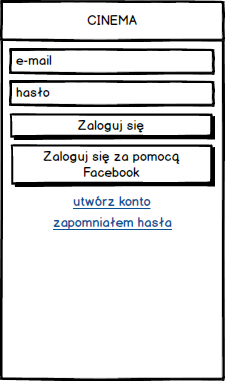
\includegraphics[width=.7\linewidth]{1}
  \captionof{figure}{Ekran logowania}
  \label{logowanie}
\end{minipage}%
\begin{minipage}{.5\textwidth}
  \centering
  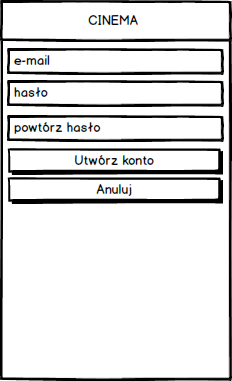
\includegraphics[width=.7\linewidth]{2}
  \captionof{figure}{Ekran rejestracji}
  \label{rejestracja}
\end{minipage}
\end{figure}

Rysunek \ref{logowanie} przedstawia ekran logowania aplikacji składający się z dwóch pól - jednego na adres e-mail, drugiego na hasło. Pole na adres e-mail jest sprawdzane pod kątem poprawności adresu e-mail, natomiast pole na hasło pokazuje wpisywany tekst w postaci gwiazdek ze względów bezpieczeństwa. Pod formularzem znajdują się przyciski. Pierwszy z nich służy do logowania za pomocą adresu e-mail i hasła. Drugi umożliwia logowanie za pomocą portalu Facebook. Dokonuje się wtedy przekierowanie do strony internetowej portalu Facebook w celu pobrania poświadczeń użytkownika. Następne dwa przyciski prowadzą odpowiednio na widok utworzenia nowego konta oraz formularza odzyskiwania hasła.

Rysunek \ref{rejestracja} przedstawia ekran rejestracji składający się z trzech pól - jednego na adres e-mail, oraz następnych dwóch na hasło. Pole na adres e-mail jest sprawdzane pod kątem poprawności adresu e-mail, natomiast pola na hasło pokazuje wpisywany tekst w postaci gwiazdek ze względów bezpieczeństwa. Pod formularzem znajdują się przyciski. Pierwszy z nich wyzwala proces tworzenia konta na podstawie podanych danych, drugi anuluje proces tworzenia konta.

\begin{figure}[h]
\centering
\begin{minipage}{.55\textwidth}
  \centering
  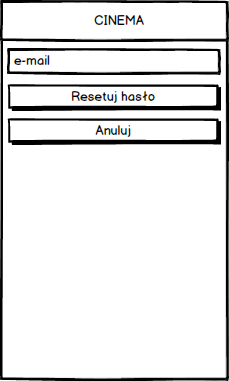
\includegraphics[width=.7\linewidth]{3}
  \captionof{figure}{Ekran resetowania hasła}
  \label{resetujhaslo}
\end{minipage}%
\begin{minipage}{.45\textwidth}
  \centering
  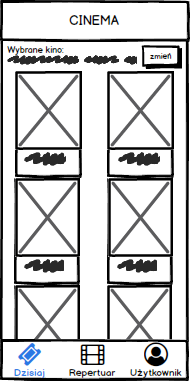
\includegraphics[width=.7\linewidth]{4}
  \captionof{figure}{Ekran z dzisiejszym repertuarem}
  \label{dzisajrepertuar}
\end{minipage}
\end{figure}

Rysunek \ref{resetujhaslo} przedstawia ekran służący do resetowania hasła składający się z jednego pola na adres e-mail. Pole na adres e-mail jest sprawdzane pod kątem poprawności adresu e-mail. Pod formularzem znajdują się przyciski. Pierwszy z nich wyzwala proces resetowania hasła na podstawie podanego adresu e-mail, drugi anuluje proces resetowania hasła.

Rysunek \ref{dzisajrepertuar} przedstawia ekran wyświetlający repertuar obowiązujący w danym kinie w dniu dzisiejszym. Na górze ekranu jest wyświetlona informacja o aktualnie wybranym kinie oraz przycisk umożliwiający zmianę kina. Poniżej znajduje się lista filmów w formie siatki. W jednym rzędzie znajdują się dwa elementy - dla większych rozdzielczości można zwiększyć liczbę elementów do trzech. Każdy element zawiera obrazek z okładką filmu, tytuł filmu oraz reżysera. Po kliknięciu w dany element, wyświetlany jest widok z informacjami o wybranym filmie. Jako, że ten widok jest częścią głównego widoku aplikacji, na dole znajduje się menu, które umożliwia szybkie i płynne przejście do szczegółowego widoku repertuaru oraz informacji o użytkowniku. 
\newpage
\begin{figure}[h]
\centering
\begin{minipage}{.5\textwidth}
  \centering
  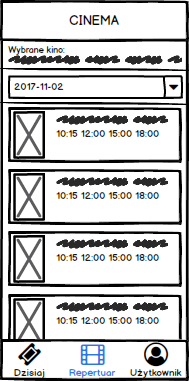
\includegraphics[width=.7\linewidth]{12}
  \captionof{figure}{Ekran szczegółowego widoku repertuaru}
  \label{repertuar}
\end{minipage}%
\begin{minipage}{.5\textwidth}
  \centering
  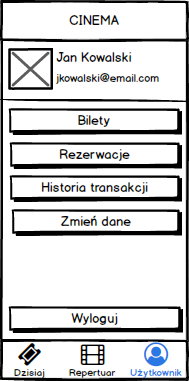
\includegraphics[width=.7\linewidth]{13}
  \captionof{figure}{Ekran użytkownika}
  \label{uzytkownik}
\end{minipage}
\end{figure}

Rysunek \ref{repertuar} przedstawia ekran z repertuarem obowiązującym w danym kinie. Na górze ekranu jest wyświetlona informacja o aktualnie wybranym kinie oraz przycisk umożliwiający zmianę kina. Poniżej znajduje się lista rozwijana umożliwiająca zmianę dnia, dla którego użytkownik chce zobaczyć repertuar. Poniżej znajduje się lista filmów. Każdy element listy zawiera obrazek z okładką filmu, tytuł filmu, reżysera oraz godziny seansów. Po kliknięciu w dany element, wyświetlany jest widok z informacjami o wybranym filmie.

Rysunek \ref{uzytkownik} przedstawia ekran użytkownika. Na górze ekranu jest wyświetlone avatar użytkownika (jeżeli dostępne), imię i nazwisko oraz adres e-mail. Poniżej znajdują się przyciski:
\begin{itemize}
\item ``Bilety`` - prowadzi do widoku aktywnych biletów
\item ``Rezerwacje`` - prowadzi do widoku aktywnych rezerwacji
\item ``Historia transakcji`` - prowadzi do widoku historii transakcji
\item ``Zmień dane`` - prowadzi do widoku zmiany danych użytkownika
\item ``Wyloguj`` - wylogowuje aktualnie zalogowanego użytkownika i prowadzi do widoku logowania.
\end{itemize}

\newpage
\begin{figure}[h]
\centering
\begin{minipage}{.5\textwidth}
  \centering
  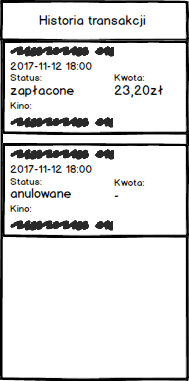
\includegraphics[width=.7\linewidth]{17}
  \captionof{figure}{Ekran historii transakcji}
  \label{historia}
\end{minipage}%
\begin{minipage}{.5\textwidth}
  \centering
  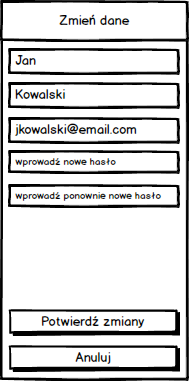
\includegraphics[width=.7\linewidth]{14}
  \captionof{figure}{Ekran zmiany danych użytkownika}
  \label{zmiana}
\end{minipage}
\end{figure}
Rysunek \ref{historia} przedstawia widok listy historycznych transakcji. Każdy element zawiera informacje o tytule filmu, datę i godzinę seansu, informacje o kinie, w którym seans się odbywał, status transakcji oraz informacje o kwocie transakcji (w przypadku braku informacji - transakcja była rezerwacją).

Rysunek \ref{zmiana} przestawia widok pozwalający na zmianę danych obecnie zalogowanego użytkownika. Składa się z formularza zawierającego informacje o imieniu, nazwisku, adresu e-mail oraz pola do zmiany hasła. Pod formularzem znajdują się przyciski - pierwszy wywołuje zmianę danych, drugi anuluje procedurę zmiany danych.
\newpage
\begin{figure}[h]
\centering
\begin{minipage}{.5\textwidth}
  \centering
  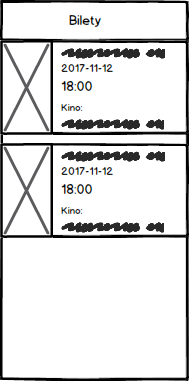
\includegraphics[width=.7\linewidth]{15}
  \captionof{figure}{Ekran aktywnych biletów}
  \label{bilety}
\end{minipage}%
\begin{minipage}{.5\textwidth}
  \centering
  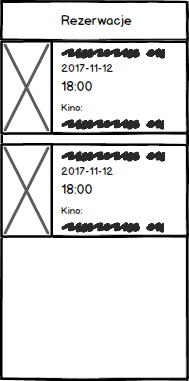
\includegraphics[width=.7\linewidth]{16}
  \captionof{figure}{Ekran aktywnych rezerwacji}
  \label{rezerwacje}
\end{minipage}
\end{figure}

Rysunki \ref{bilety} oraz \ref{rezerwacje} pokazują widoki z listą aktywnych biletów oraz rezerwacji. Każdy element zawiera informacje o tytule filmu, obrazek z okładką filmu, datę i godzinę seansu oraz informacje o kinie w którym seans się odbywa. Po kliknięciu w dany element, użytkownik jest kierowany na stronę ze szczegółami odpowiednio biletu oraz rezerwacji.

\newpage
\begin{figure}[h]
\centering
\begin{minipage}{.5\textwidth}
  \centering
  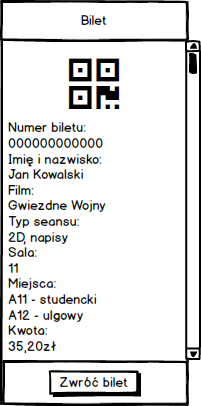
\includegraphics[width=.7\linewidth]{18}
  \captionof{figure}{Ekran szczegółów biletu}
  \label{bilet}
\end{minipage}%
\begin{minipage}{.5\textwidth}
  \centering
  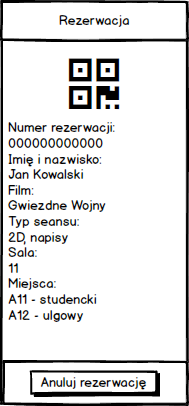
\includegraphics[width=.65\linewidth]{19}
  \captionof{figure}{Ekran szczegółów rezerwacji}
  \label{rezerwacja}
\end{minipage}
\end{figure}

Rysunki \ref{bilet} oraz \ref{rezerwacja} przedstawiają widok szczegółowy biletu oraz rezerwacji. Na samej górze znajduje się wygenerowany kod QR, umożliwiający szybkie odnalezienie biletu/rezerwacji w systemie oraz szybką kontrolę biletów. Pod kodem QR znajdują się szczegóły:  numer identyfikujący, imię i nazwisko osoby zawierającej transakcję, nazwa filmu, data i godzina seansu, typ seansu, kino oraz sala w której odbywa się seans, lista zarezerwowanych miejsc oraz, w przypadku biletu, kwota jaką uiszczono. Na dole znajdują się przyciski umożliwiające rozpoczęcie procedury zwrotu biletu lub anulowania rezerwacji.

\newpage
\begin{figure}[h]
\centering
\begin{minipage}{.5\textwidth}
  \centering
  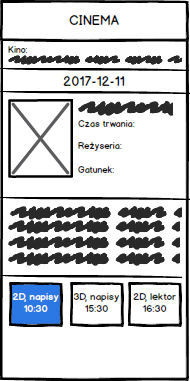
\includegraphics[width=.7\linewidth]{5}
\end{minipage}%
\begin{minipage}{.5\textwidth}
  \centering
  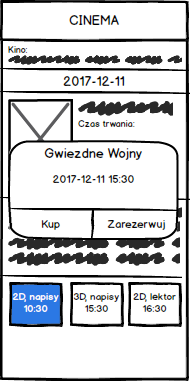
\includegraphics[width=.7\linewidth]{6}
\end{minipage}
\caption{Ekran informacji o filmie}
\label{info}
\end{figure}

Rysunek \ref{info} przedstawia ekran wyświetlający informacje o wybranym filmie. Na górze wyświetlone jest informacja o aktualnie wybranym kinie, poniżej dzień dla którego wyświetlane są informacje o seansach. Następnie są widoczne informacje o filmie: obrazek z plakatem filmu, tytuł filmu, czas trwania, informacje o reżyserze, gatunku oraz krótki opis. Pod opisem znajduje się lista seansów w danym dniu w formie siatki. Po wybraniu jednego z seansów wyświetla się komunikat z prośbą o sprecyzowanie operacji jaką chce wykonać użytkownik: czy chce dokonać zakupu czy rezerwacji. Po wybraniu operacji, użytkownik jest kierowany na ekran widoku sali.
\newpage
\begin{figure}[h]
\centering
\begin{minipage}{.5\textwidth}
  \centering
  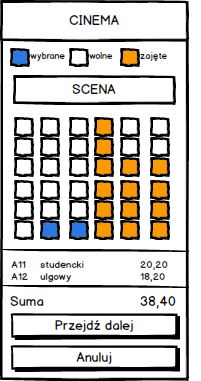
\includegraphics[width=.7\linewidth]{7}
\end{minipage}%
\begin{minipage}{.5\textwidth}
  \centering
  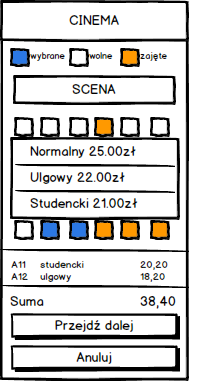
\includegraphics[width=.7\linewidth]{8}
\end{minipage}
\caption{Ekran widoku sali}
\label{sala}
\end{figure}

Rysunek \ref{sala} przedstawia ekran z widokiem sali. Składa się z części umożliwiającej wybór miejsc na sali, informacji o wybranych przez użytkownika miejscach oraz przycisków, które odpowiednio: kierują użytkownika na widok podsumowania transakcji oraz anulują transakcję. W przypadku kupowania biletu, po wyborze miejsca wyświetla się monit o wyborze rodzaju biletu.

\newpage
\begin{figure}[h]
\centering
\begin{minipage}{.33\textwidth}
  \centering
  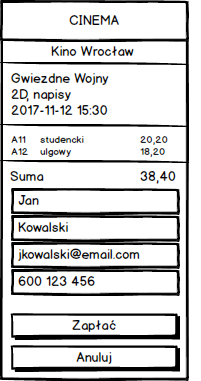
\includegraphics[width=.7\linewidth]{9}
\end{minipage}%
\begin{minipage}{.33\textwidth}
  \centering
  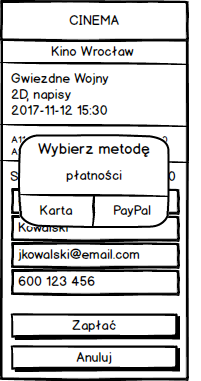
\includegraphics[width=.7\linewidth]{10}
\end{minipage}
\begin{minipage}{.33\textwidth}
  \centering
  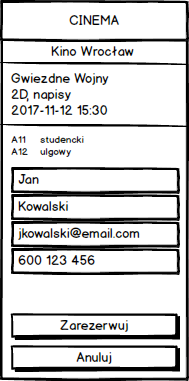
\includegraphics[width=.7\linewidth]{11}
\end{minipage}
\caption{Ekran podsumowania transakcji}
\label{podsumowanie}
\end{figure}

Rysunek \ref{podsumowanie} przedstawia widok podsumowania transakcji. Znajdują się na nim informacje takie jak: kino w którym odbędzie się wybrany seans, tytuł filmu, rodzaj seansu, data i godzina seansu, lista wybranych miejsc oraz formularz z danymi użytkownika. W dolnej części ekranu znajdują się przyciski do potwierdzenia oraz anulowania transakcji. W przypadku zakupu biletów, po potwierdzeniu wyświetla się monit z prośbą o wybór metody płatności.
\newpage
\section{Diagram klas}
\addtocontents{toc}{\protect\newpage}
W tym rozdziale zostały przedstawione diagramy klas uwzględniające najważniejsze aspekty projektu.
\begin{figure}[h]
\centering
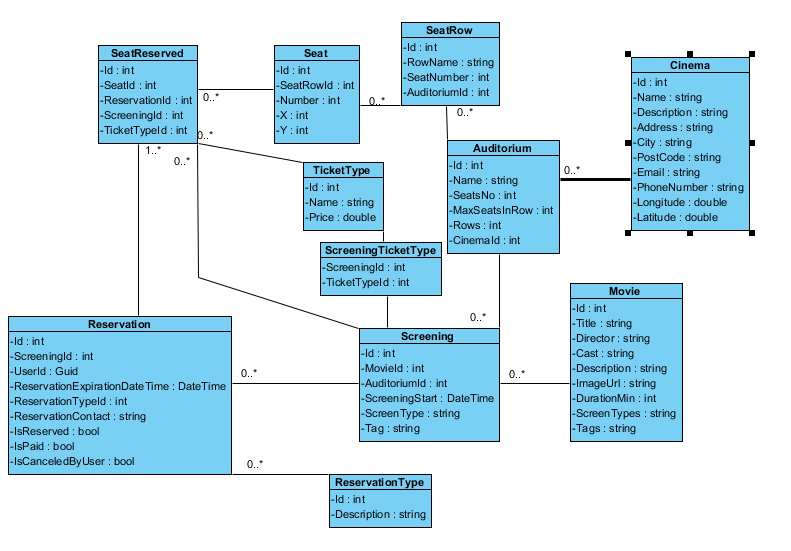
\includegraphics[width=1\textwidth]{100}
\caption{Diagram klas opisujących encje}
\label{klasy1}
\end{figure}
\par
Rysunek \ref{klasy1} przedstawia diagram klas opisujących główne encje w projekcie. Klasa Cinema opisuje pojedynczą instancję kina. Zawiera podstawowe informacje o kinie. Klasa Cinema może posiadać wiele obiektów klasy Auditorium - opisuje ona informacje o sali kinowej. Klasa Auditorium może zawierać wiele obiektów klasy SeatRow - jest to klasa opisująca rząd siedzeń, a z kolei klasa SeatRow zawiera wiele obiektów klasy Seat, która opisuje pojedyncze miejsce na sali.

Klasa Screening jest klasą opisującą pojedynczy seans filmowy. Ma ona przypisaną salę (Auditorium) oraz film (klasa Movie). Klasa Reservation opisuje informacje o rezerwacji. Ma przypisany seans (Screening) oraz typ rezerwacji (ReservationType). Zarezerwowane miejsca opisuje klasa SeatReserved, która zawiera odniesienia do klas Reservation, Seat, TicketType oraz Screening. Oprócz tego jest jeszcze klasa agregująca ScreeningTicketType, która została stworzona w celu wymuszenia relacji wiele-do-wielu w Entity Framework Core.
\newpage
\begin{figure}[h]
\centering
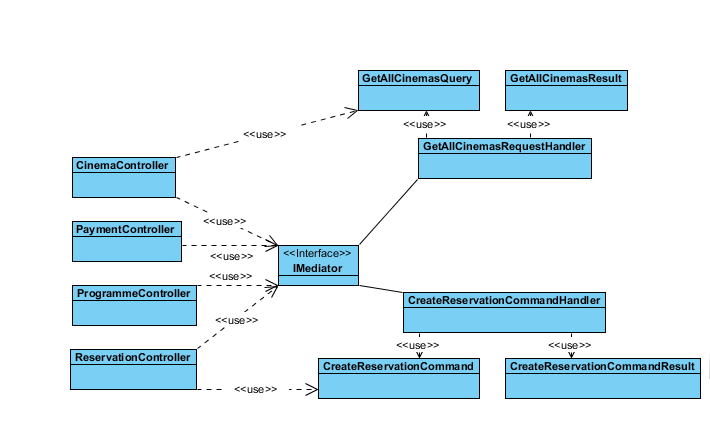
\includegraphics[width=1\textwidth]{101}
\caption{Diagram klas opisujący kontrolery oraz wykorzystanie wzorca Mediator}
\label{klasy2}
\end{figure}
Rysunek \ref{klasy2} przedstawia diagram klas opisujących kontrolery w aplikacji webowej oraz wykorzystanie wzorca Mediator. Z racji dużej ilości klas obsługującej komendy oraz zapytania, diagram klas zawiera dwie przykładowe klasy. Kontrolery wykorzystują obiekt mediatora (mediator jest wstrzykiwany jako zależność) i przekazują do niego odpowiedni obiekt, który potem z pomocą mediatora jest kierowany do odpowiedniego handlera. Dla przykładu kontroler CinemaController przekazuje do mediatora obiekt typu GetAllCinemasQuery, który dalej jest przekazywany do obiektu klasy GetAllCinemasRequestHandler. Wykorzystanie mediatora jest ściśle powiązane z implementacją wzorca CQRS (więcej o tym wzorcu w podrozdziale \ref{sec:cqrs})
\newpage
\begin{figure}[h]
\centering
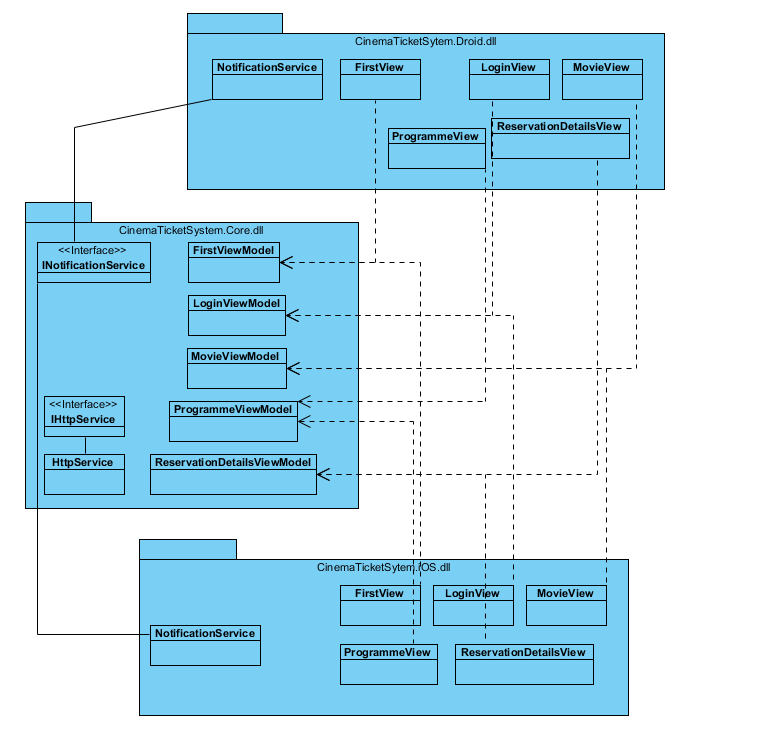
\includegraphics[width=0.8\textwidth]{102}
\caption{Diagram klas opisujący wykorzystanie wzorca Model-View-Viewmodel}
\label{klasy3}
\end{figure}
Rysunek \ref{klasy3} przedstawia diagram klas przedstawiający zamysł architektury Model-View-ViewModel. W tej architekturze następuje wyraźny podział odpowiedzialności pomiędzy widokiem, modelem, a widokiem modelu. Widok jest graficzną częścią aplikacji. Widok modelu obsługuje wszystkie akcje, które są połączone z widokiem oraz eksponuje dane z modelu dla widoku. W modelu znajduje się logika aplikacji. Dzięki oddzieleniu logiki aplikacji od widoku możliwe jest współdzielenie większości kodu pomiędzy aplikacje dla dwóch platform. Na tym przykładzie biblioteka CinemaTicketSystem.Core.dll zawiera wszystkie modele widoku, modele oraz serwisy. Dzięki temu w aplikacjach na konkretne platformy jest jedynie potrzeba stworzenia odpowiednich widoków oraz powiązanie ich z akcjami w odpowiadających im modelach widoku. W przypadku konieczności wykorzystania specyficznych dla danej platformy funkcjonalności można stworzyć interfejs serwisu w bibliotece Core, oraz odpowiednie jego implementacje w poszczególnych aplikacjach. Za poprawne rozwiązywanie zależności dba tutaj kontener IoC (odwrócenie sterowania ang. \textit{inversion of control})
\chapter{Implementacja}
W tym rozdziale zostały opisane najważniejsze aspekty dotyczące fazy implementacji. Pierwszy podrozdział opisuje wykorzystanie metodyki DevOps w celu zapewnienia jakości produktu końcowego. W drugim podrozdziale zawarte jest rozwiązanie problemu autoryzacji użytkowników aplikacji mobilnej. W dalszej części znajdują się: opis zastosowanych technik mających na celu zapewnienie bezpieczeństwa aplikacji, sposób i cel wykorzystania wzorca CQRS (\textit{Command Query Responsibility Segregation}) oraz opis przeprowadzonych testów interfejsu użytkownika.
\section{DevOps}
DevOps (\textit{development and operations}) jest to sposób wytwarzania oprogrmowania, mający na celu ścisłą współpracę pomiędzy osobami (programistami) odpowiedzialnymi za rozwój oprogramowania, a osobami specjalizującymi się w utrzymywaniu rozwiązań IT (administratorzy). Dzięki ścisłej współpracy grup osób odpowiedzialnych za rozwój (\textit{development}), eksploatację (\textit{operations}) oraz zapewnienie jakości (\textit{quality assurance}), DevOps znacznie skraca czas wdrożenia nowych funkcji w oprogramowaniu. Temat DevOps został po raz pierwszy zaprezentowany w 2009 roku przez Patricka Debois w trakcie pierwszej konferencji DevOps Days w Belgii. \cite{RefWorks:2}\cite{Czymjest19:online}

Metoda DevOps jest obecnie wykorzystywana głównie przez firmy i organizacje, które wytwarzają i wdrażają dużą ilość zmian w swoim oprogramowaniu, działającym na środowiskach produkcyjnych przy zachowaniu jak najkrótszego czasu potrzebnego na wdrożenie oraz wysokiej jakości oprogramowania. \cite{Devopsco42:online}
\newpage
Pojęcie DevOps jest ściśle powiązane z procesami takimi jak:
\begin{itemize}
\item Continuous Integration (ciągła integracja),
\item Continuous Delivery (ciągłe dostarczanie),
\item Continuous Testing (ciągłe testowanie),
\item Continuous Monitoring (ciągły monitoring) oraz
\item Continuous Deployment (ciągłe wdrażanie)
\end{itemize}
Definiują one w klarowny sposób jakie procesy są realizowane w ramach metodyki DevOps. Innymi słowy, DevOps można przedstawić jako pewien rodzaj dyscypliny w budowie oraz weryfikacji wytwarzanego oprogramowania, za pośrednictwem testów regresji oraz statycznej analizy kodu zawartego w systemie kontroli wersji (pokrycie kodu testami, ocena długu technologicznego). To podejście jest jedną z najbardziej zwinnych praktyk rozwoju oprogramowania. Umożliwia opracowanie rozwiązań wysokiej jakości, zapewniając aktualną informację zwrotną na temat wad wytworzonego kodu. \cite{Devopsco42:online}

\begin{figure}[h]
\centering
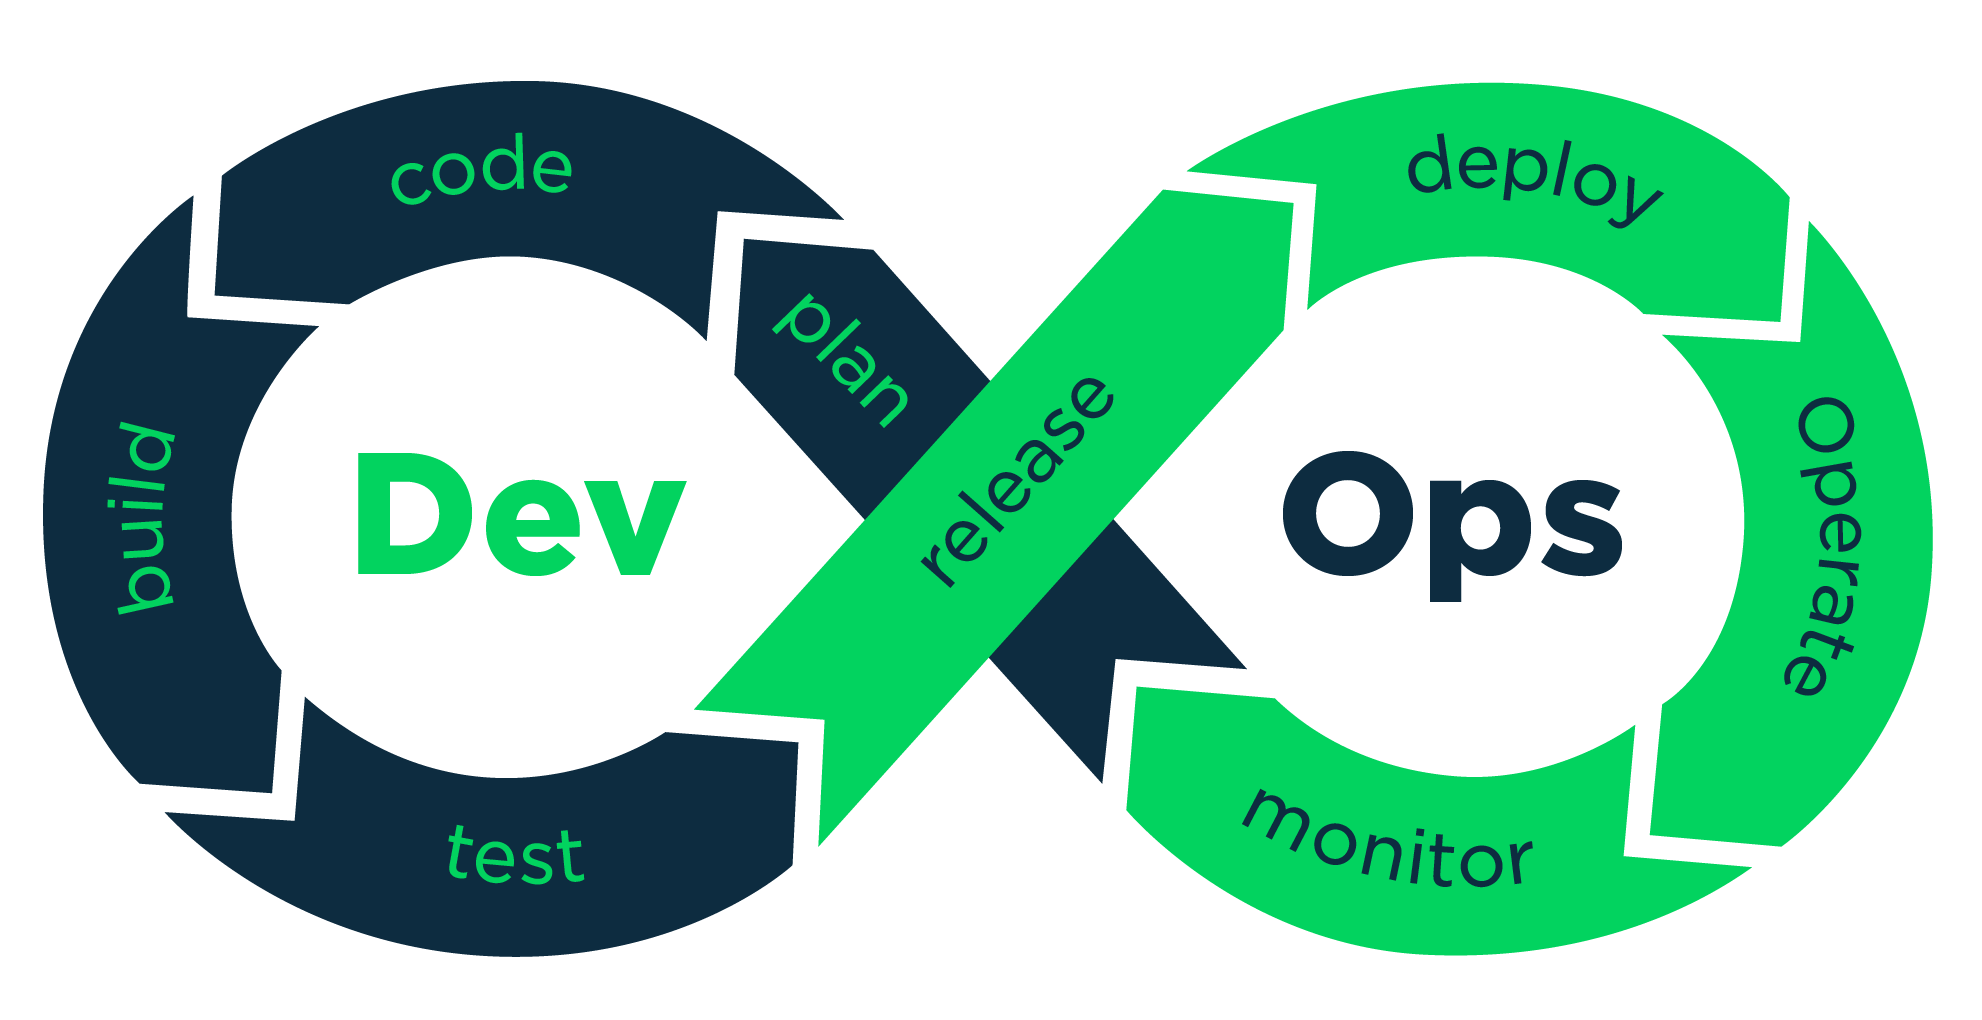
\includegraphics[width=0.7\textwidth]{img2}
\caption{Wizualizacja procesu wytwarzania oprogramowania w ramach metodyki DevOps}
(źródło: opracowanie własne)
\end{figure}

W procesie wytwarzania opisywanego systemu została wykorzystana opisana wyżej metodyka, w celu zapewnienia jakości oprogramowania. Do planowania prac został wykorzystany system Team Foundation Server wspierający podejście zwinne (\textit{Agile}) do prowadzenia projektu. (opisany w podrozdziale \ref{sec:team}). Zadania były definiowane jako historyjki użytkownika powstałe podczas tworzenia wymagań funkcjonalnych. Do każdego takiego zadania tworzono podzadania (ang. \textit{subtasks}) opisujące techniczne aspekty uzyskania danej funkcjonalności. W późniejszym etapie funkcjonowania systemu, TFS może być wykorzystywany do przechowywania informacji o zgłoszonych przez użytkowników (testerów oraz użytkowników końcowych) błędach oraz propozycjach zmian.

W kroku implementacji rozwiązania wykorzystano repozytoria systemu kontroli wersji Git, którego obsługę wbudowano w Team Foundation Server. W ramach projektu utworzono dwa repozytoria. Osobne dla aplikacji serwerowej oraz mobilnej. W ramach pracy nad konkretnymi funkcjonalnościami, wykorzystano mechanizmy oferowane przez wyżej wymieniony system kontroli wersji  m.in.: \textit{feature branches}, \textit{pull requests}. Ma to bardzo duże znaczenie w przypadku projektów zespołowych, pozwalajac na bezproblemowy, równoległy rozwój oprogramowania.

W następnym kroku następuje budowanie rozwiązania w ramach ciągłej integracji. Po wykonaniu zmian w repozytorium kodu (w głównej gałęzi - w branchu master) następuje automatyczne budowanie projektów na serwerze budującym działającym w chmurze Microsoft Azure jako maszyna wirtualna, opartym o system Windows Server 2016. Serwer budujący jest zintegrowany z systemem Team Foundation Server co umożliwia łatwe tworzenie definicji budowania. 

Po pomyślnie ukończonym procesie budowania rozwiązania, uruchamiane są testy jednostkowe oraz statyczna analiza kodu z wykorzystaniem NDepend. Dzięki temu natychmiast uzyskujemy statystyki dotyczące pokrycia kodu testami (ang. \textit{code coverage}) oraz prognozowanego długu technologicznego (ang. \textit{technical debt}).

W następnym kroku udostępniane są artefakty powstałe podczas procesu budowania oraz:
\begin{itemize}
\item w przypadku aplikacji serwerowej następuje wdrożenie aplikacji na środowisko deweloperskie utworzone w usłudze Microsoft Azure - po ukończeniu testów na środowisku deweloperskim, po ręcznym zaakceptowaniu przez uprawnionego użytkownika, następuje wdrożenie na środowiska \textit{staging} oraz produkcyjne
\item w przypadku aplikacji mobilnej następuje dystrybucja aplikacji do testerów w ramach systemu Visual Studio Mobile Center jako wersja alpha (więcej o VS Mobile Center w podrozdziale \ref{sec:hockeyapp}) - po ukończeniu testów wersji alpha, po ręcznym zaakceptowaniu przez uprawnionego użytkownika, następuje dystrbucja aplikacji w wersji beta dla szerszego grona testerów oraz wersji produkcyjnej do internetowych sklepów takich jak Google Play Store oraz Apple App Store
\end{itemize}

Do zbierania telemetrii aplikacji zastosowano usługi: Azure Application Insights dla aplikacji serwerowej oraz Visual Studio Mobile Center dla aplikacji mobilnych. Dzięki wyżej wymienionym usługom, mamy dostęp do wielu statystyk takich jak np.: średni czas odpowiedzi serwera, ilość żądań HTTP, czas uruchamiania aplikacji, statystyki dotyczące urządzeń korzystających z aplikacji, dane dotyczące wyjątków, które wystąpiły w trakcie działania aplikacji. Dzięki integracji z Team Foundation Server jest możliwe automatyczne tworzenie zgłoszeń o błędach w aplikacji na podstawie wystepujących wyjątków.
\section{Uwierzytelnianie i autoryzacja użytkowników aplikacji}
Aspekt autoryzacji użytkowników aplikacji jest to jeden z najbardziej powszechnych problemów przy tworzeniu systemów informatycznych. Odpowiedni wybór mechanizmu autoryzacji, uwierzytelniania oraz zarządzania uprawnieniami użytkowników jest często kluczowy jeśli chodzi o późniejsze bezpieczeństwo aplikacji. W zależności od rodzaju tworzonej aplikacji stosuje się różne metody uwierzytelniania i autoryzacji. 

Dla klasycznych aplikacji webowych stosuje się zazwyczaj podejście z wykorzystaniem plików cookie. Użytkownik próbujący się dostać do zabezpieczonego zasobu, zostaje przekierowany do strony logowania w przypadku nie posiadania prawidłowego pliku cookie z danymi o sesji. Strona logowania, po zweryfikowaniu podanych danych poświadczających (zazwyczaj stosowana jest uwierzytelnianie z wykorzystaniem loginu i hasła - \textit{Challenge–response authentication}), zapisuje w przeglądarce plik cookie, który jest potem wykorzystywany przy żądaniach do zabezpieczonych zasobów, w ramach tej samej przeglądarki do czasu wygaśnięcia pliku.

Trochę inaczej to wygląda w przypadku aplikacji webowych typu \textit{Single Page Application} oraz aplikacji mobilnych. Mamy zazwyczaj wtedy do czynienia z aplikacją serwerową działającą jako WebAPI (API - \textit{application programming interface}) oraz aplikacjami klienckimi (SPA, aplikacja mobilna), która łączy się z aplikacją serwerową w celu pobrania wymaganych danych. Uwierzytelnianie polega na wysłaniu przez aplikację kliencką danych uwierzytelniających (może to być para login-hasło, ale również poświadczenia uzyskane od zewnętrznych dostawców takich jak Facebook, Google itp.) do serwera autoryzującego, który w przypadku poprawności wysłanych danych, odsyła do klienta \textit{access token} oraz \textit{refresh token}. Access token jest wysyłany wraz z każdym żądaniem do serwera, natomiast refresh token służy do odnawiania access tokena.

Taki mechanizm jest podyktowany tym, że access token ma zazwyczaj bardzo krótki czas ważności (np. 30 minut). Jest to celowe, ponieważ w przypadku dłuższego czasu ważności access tokena powstaje problem spowodowany tym, że teoretycznie nie ma możliwości unieważnienia tokena przed czasem wygaśnięcia. Wyobraźmy sobie, że jest użytkownik z rolą ,,Administrator'', która została w pewnym momencie zmieniona na rolę ,,Użytkownik''. W takiej sytuacji, użytkownik posiadający token ze starą rolą ,,Administrator'' ma dostęp do zasobów dostępnych tylko dla Administratora do czasu wygaśnięcia tokena. Drugi z tokenów ma natomiast dłuższy okres ważności (np. 1 rok) - dzięki temu po wygaśnięciu access tokena, mamy możliwość wygenerowanie nowej pary tokenów bez potrzeby ponownego uwierzytelniania.
\newpage
Otrzymane tokeny zostają zapisane przez klienta w celu późniejszego wykorzystania. W aplikacjach typu SPA, tokeny są zapamiętywane w \textit{local storage} lub \textit{session storage} przeglądarki (interfejs \textit{HTML5 Web Storage}), natomiast w aplikacjach mobilnych w wewnętrznej pamięci urządzenia. 

\begin{figure}[h!]
\centering
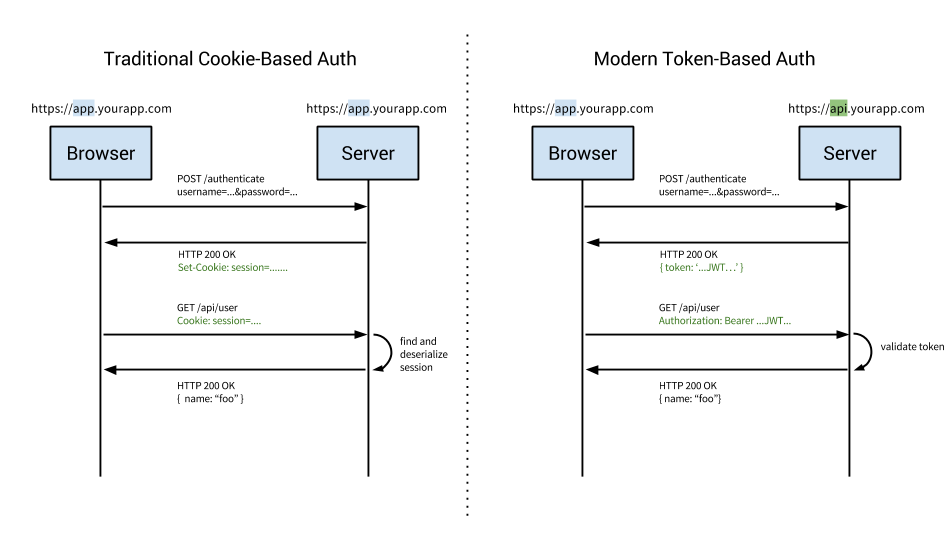
\includegraphics[width=0.9\textwidth]{img3}
\caption{Porównanie mechanizmów uwierzytelniania z wykorzystaniem plików cookie oraz tokenów}
(źródło: https://auth0.com/blog/cookies-vs-tokens-definitive-guide/)
\end{figure}

Po uzyskaniu \textit{access tokena}, użytkownik może wysyłać żądania do zabezpieczonych zasobów dodając do żądania nagłówek \textit{Authorization} i jako typ nagłówka \textit{Bearer}. Cały nagłówek wygląda według wzoru: \textit{Authorization: Bearer <<access token>>} Po pomyślnym zweryfikowaniu tokena, następuje wysłanie przez serwer żądanych informacji. W przypadku gdy access token okaże się nieważny, serwer zwraca błąd HTTP 401 Unauthorized. Jest to informacja dla aplikacji klienckiej, że należy spróbować uzyskać nowy access token za pomocą refresh tokena.

\subsection*{Realizacja uwierzytelniania i autoryzacji w aplikacji}
\label{autory}
Uwierzytelnianie oraz autoryzacja zostały zaimplementowane z wykorzystaniem podejścia tokenowego. Framework Identity Server 4 (podrozdział \ref{sec:is4}) umożliwia zabezpieczenie w szybki sposób WebAPI stworzonego w ASP.NET Core. Dzięki integracji z wbudowanym mechanizmem ASP.NET Core Identity uzyskujemy pełny mechanizm uwierzytelniania, autoryzacji oraz zarządzania kontami i rolami użytkowników w pełni zgodny z protokołem OAuth 2.0.
\newpage
Użytkownik może uwierzytelniać się na dwa sposoby:
\begin{itemize}
\item z wykorzystaniem loginu i hasła
\item z wykorzystaniem poświadczeń uzyskanych od zewnętrznego dostawcy - Facebook
\end{itemize}

Przepływ procesu dla pierwszego ze sposobów wygląda następująco:
\begin{enumerate}
\item Użytkownik podaje w aplikacji klienckiej login i hasło do swojego konta
\item Aplikacja wysyła żądanie do serwera autoryzującego
\item W przypadku poprawnego uwierzytelnienia, serwer wysyła do klienta parę tokenów - access token oraz refresh token. Oba tokeny są w formacie JWT (JSON Web Token)
\item Oba tokeny zostają zapisane w pamięci urządzenia mobilnego
\item Aplikacja dodaje access token do żądania HTTP w nagłówku Authorization
\item W przypadku pozytywnej weryfikacji tokena, serwer zwraca żądane przez użytkownika dane.
\end{enumerate}
Przepływ procesu dla drugiego ze sposobów wygląda następująco:
\begin{enumerate}
\item Użytkownik loguje się na swoje konto u zewnętrznego dostawcy
\item Zewnętrzny dostawca zwraca do klienta access token.
\item Klient wysyła otrzymany access token do serwera autoryzującego
\item Serwer autoryzujący sprawdza poprawność access tokena u zewnętrznego dostawcy i w razie powodzenia zwraca wygenerowaną parę tokenów. Oba tokeny są w formacie JWT (JSON Web Token)
\item Oba tokeny zostają zapisane w pamięci urządzenia mobilnego
\item Aplikacja dodaje access token do żądania HTTP w nagłówku Authorization
\item W przypadku pozytywnej weryfikacji tokena, serwer zwraca żądane przez użytkownika dane.
\end{enumerate}
\subsection*{JSON Web Token}
Wspomniany powyżej JSON Web Token jest to rodzaj tokenu przechowywanego u klienta. Jest on w formacie JSON, jak wskazuje jego nazwa. Token jest szyfrowany po stronie serwera i tylko serwer ma klucz dający możliwość zweryfikowania autentyczności tokenu.

JWT składa się z trzech części. Wszystkie dane są zakodowane przez algorytm Base64 i dopiero w takiej postaci przechowywane.
\begin{itemize}
\item Header - tutaj jest przechowywana informacja o algorytmie szyfrującym wykorzystanym przy generowaniu tokenu.
\item Payload - są to dane, które chcemy przechowywać po stronie klienta. Nie są one zaszyfrowane. Z reguły są to dane dotyczące użytkownika takie jak jego identyfikator czy też informacje o uprawnieniach. Dzięki temu mamy szybki dostęp do najczęściej potrzebnych danych po stronie klienta
\item Signature - podpis cyfrowy, będący zaszyfrowanym połączeniem poprzednich dwóch części. Serwer po otrzymaniu tokenu, odszyfrowuje tą część i porównuje dane z częścią Payload i dopiero w przypadku stwierdzenia poprawności danych, przepuszcza zapytanie jako prawidłowe
\end{itemize}

Zastosowanie JSON Web Token pozwala również ograniczyć ilość zapytań do serwera oraz bazy danych. Przy logowaniu są pobierane takie dane jak na przykład identyfikator użytkownika, jego role, imię oraz nazwisko, które aplikacja zapisuje w swojej pamięci, co wiąże się z tym że nie ma potrzeby pobierania tych danych za każdym razem kiedy pojawiają się one w widoku. Poprawność danych zapewnia nam podpis cyfrowy zawarty w tokenie.

\newpage
\section{Bezpieczeństwo aplikacji}
W przypadku aplikacji, które operują na danych osobowych oraz oferują integrację z systemem płatności, bardzo ważnym aspektem jest jej bezpieczeństwo. Tego typu aplikacje powinny spełniać szereg norm.

Pierwszą rzeczą, która została wprowadzona do aplikacji jest wymuszenie szyfrowanego ruchu pomiędzy klientem i serwerem na środowisku produkcyjnym. Takie zabezpieczenie zmniejsza ryzyko skutecznego przechwycenia żądania do serwera w trakcie korzystania z otwartych sieci Wi-Fi. Atakujący jest w stanie przechwycić takie żądanie, ale ze względu na szyfrowanie - nie jest on zwykle uzyskać z niego żadnych informacji.

Następnym usprawnieniem w kontekście bezpieczeństwa jest rozproszenie danych. Baza danych przechowująca dane klientów, znajduje się na innym serwerze niż baza zawierająca dane dotyczące rezerwacji. (patrz rozdział \ref{fizy}).

Wszystkie dane są przechowywane na serwerach platformy obliczeniowej Microsoft Azure, która musi spełniać najwyższe standardy europejskie w kontekście bezpieczeństwa danych osobowych. Serwery te znajdują się na terenie jednego z państw członkowskich Unii Europejskiej. Zmniejsza to znacznie ryzyko fizycznego wykradzenia danych klientów (fizyczny dostęp do serwera jest praktycznie niemożliwy).

Uwierzytelnianie oraz autoryzacja użytkowników odbywa się za pośrednictwem JSON Web Token. (więcej o JSON Web Token w podrozdziale \ref{autory}) Dzięki przesyłaniu danych w formie hasza, możliwości sprawdzenia autentyczności tokena z pomocą podpisu cyfrowego oraz późniejszej walidacji tokena przez serwer autoryzujący, zmniejsza się ryzyko podszycia się pod innego użytkownika i uzyskania dostępu do jego wrażliwych danych.

Innym zabezpieczeniem aplikacji jest obfuskacja kodu aplikacji na platformę Android z wykorzystaniem mechanizmu ProGuard. Zaciemniony kod jest trudniejszy do uzyskania w ramach inżynierii odwrotnej oraz trudniejszy w interpretacji. ProGuard zmienia nazwy klas, pól oraz metod na semantycznie niejasne nazwy oraz usuwa nieużywany kod.

W przypadku aplikacji na system iOS, zaciemnienie kodu nie jest konieczne ze względu na rygorystyczne zabezpieczenia DRM firmy Apple, które szyfrują pewną część aplikacji, dzięki czemu odzyskanie kodu źródłowego z wykorzystaniem inżynierii odwrotnej jest wyjątkowo utrudnione.
\newpage
\section{Implementacja wzorca CQRS}
\label{sec:cqrs}
\textit{Command Query Responsiblity Segregation} jest wzorcem zaproponowanym pierwszy raz przez Grega Young'a. Wzorzec ten odseparowuje operacje odczytujące dane (zapytania ang. \textit{queries}) od operacji aktualizujących dane (komendy ang. \textit{commands}) z wykorzystaniem osobnych interfejsów. Bardzo często też spotyka się w tym miejscu izolację modeli służących do odczytu i modeli służących do zapisu danych.

W porównaniu z podejściem z jednym modelem danych w systemach opartych na operacjach CRUD (\textit{Create-Read-Update-Delete}), użycie osobnych modeli dla operacji odczytu i aktualizacji danych w systemach opartych na CQRS znacząco upraszcza projektowanie oraz fazę implementacji. 

Model dla odczytu danych oraz model dla aktualizacji danych mogą mieć dostęp do tej samej bazy danych. Jednak bardzo często wykorzystuje się więcej niż jedno fizyczne źródło danych w celu poprawienia wydajności, skalowalności oraz bezpieczeństwa aplikacji.

W takim podejściu źródło danych służące do odczytu jest  zazwyczaj dokładną kopią źródła danych na którym dokonujemy zmian. Bardzo często się spotyka połączenie klasycznego silnika bazodanowego (np. Microsoft SQL Server), na którym są wykonywane operacje zapisu, oraz silników wyszukiwania typu Elasticsearch umożliwiając w ten sposób bardzo szybki dostęp do danych, co jest bardzo ważne szczególnie w aplikacjach typu enterprise.

\subsubsection*{Realizacja wzorca CQRS w aplikacji}

W projekcie aplikacji zastosowano podejście z pojedynczym źródłem danych. Dla zwiększenia wydajności wykorzystywane są dwa mappery obiektowo-relacyjne (\textit{ORM}). Do zapisu danych służy Entity Framework Core, który ułatwia tworzenie operacji zapisu danych dzięki braku konieczności pisania kodu SQL oraz zaimplementowanemu wzorcowi Unit of Work. Do odczytu danych służy \textit{microORM} Dapper, który oferuje znacznie mniejszy narzut wydajnościowy w porównaniu z innymi ORMami. Jego wydajność jest niewiele gorsza niż w przypadku bezpośredniego wywoływania zapytań SQL do bazy danych.

Razem ze wzorcem CQRS wykorzystano wzorzec projektowy - mediator. Celem wykorzystania mediatora było zmniejszenie stopnia skomplikowania zależności między komponentami oraz ułatwienie tworzenia testów jednostkowych. Mediator jest klasą która zna dokładnie metody wszystkich klas, którymi zarządza. Nie muszą one wiedzieć o sobie, jedynie przekazują polecenia mediatorowi, a ten przesyła je dalej do odpowiednich obiektów. W projekcie wykorzystano bibliotekę MediatR wspierającą rozwiązania tworzone w ASP.NET Core.
\newpage
\begin{lstlisting}[caption={Przykładowa metoda kontrolera w aplikacji wykorzystującej CQRS oraz wzorzec mediatora},captionpos=b]
 public class CinemaController : Controller
    {
        private readonly IMediator _mediator;
        public CinemaController(IMediator mediator)
        {
            _mediator = mediator;
        }

        public async Task<ActionResult> GetCinema(GetAllCinemasQuery query)
        {
            var model = await _mediator.Send(query);
            return Ok(model);
        }
    }
\end{lstlisting}
\begin{lstlisting}[caption={Przykładowy model polecenia odczytu danych},captionpos=b]
 public class GetAllCinemasQuery : IRequest<GetAllCinemasResult>
    {
        public Guid DeviceId { get; set; }
    }
\end{lstlisting}
\begin{lstlisting}[caption={Przykładowy model odpowiedzi serwera},captionpos=b]
 public class GetAllCinemasResult
    {
        public IEnumerable<Cinema> Cinemas { get; set; }
    }
\end{lstlisting}
\newpage
\begin{lstlisting}[caption={Przykładowa realizacja operacji odczytu danych},captionpos=b]
 public class GetAllCinemasRequestHandler : IRequestHandler<GetAllCinemasQuery, GetAllCinemasResult>
    {
        private readonly IConfiguration _configuration;
        public GetAllCinemasRequestHandler(IConfiguration configuration)
        {
            _configuration = configuration;
        }

        public GetAllCinemasResult Handle(GetAllCinemasQuery message)
        {
            IEnumerable<Cinema> cinemas;
            using (IDbConnection db = new SqlConnection(
            _configuration.GetConnectionString("DefaultConnection")))
            {
                cinemas = db.Query<Cinema>("SELECT * FROM Cinemas;").ToList();
            }

            return new GetAllCinemasResult {Cinemas = cinemas};
        }
    }
\end{lstlisting}
\newpage
\section{Testy interfejsu aplikacji}
Przy tworzeniu systemu informatycznego, oprócz samej implementacji, bardzo ważny jest etap testowania rozwiązania. Testy jednostkowe, akceptacyjne czy też automatyczne pozwalają na zmniejszenie ilości błędów w oprogramowaniu, jeszcze przed wdrożeniem na środowisko produkcyjne.

W ramach implementacji stworzono testy automatyczne z wykorzystaniem Xamarin UI Tests, które w bardzo prosty sposób pozwalają na stworzenie zestawu testów, które sprawdzają poprawność zachowania interfejsu użytkownika. Testy tworzono dla pojedynczych widoków

Testy z wykorzystaniem Xamarin UI Tests mogą być uruchamiane na fizycznych urządzeniach podłączonych z pomocą kabla USB lub w ramach serwisów takich jak Xamarin Test Cloud, który umożliwia zdalne przetestowanie aplikacji na szerokiej palecie fizycznych urządzeń.

Testy Xamarin UI Tests bazują na bibliotece nUnit - popularnej bilbiotece wykorzystywanej do pisania testów jednostkowych.

\begin{lstlisting}[caption={Przykładowy test automatyczny z wykorzystaniem Xamarin UI Tests},captionpos=b]
[TestFixture]
public class UserLogin
{
private IApp app;
private const string apkPath = "com.cinema.apk";

	[SetUp]
	public void Setup()
	{
		app = ConfigureApp.Android.ApkFile (apkPath).StartApp();
	}

	[Test]
	[TestCase(TestName="Hello")]
	public void DoesNothing()
	{
		app.Screenshot ("This app does nothing");
	}
			
	[Test]
	[TestCase(TestName="Login")]
	public void Login()
	{
		app.Screenshot ("Given the app is running");
		app.WaitForElement(e => e.Id("emailInput"));

		app.Screenshot ("I'll provide user e-mail");
		app.EnterText(e => e.Id("emailInput"), "jkowalski@email.com");
		
		app.Screenshot ("I'll provide user password");
		app.EnterText(e => e.Id("password"), "password");

		app.Screenshot ("And I want to login.");
		app.Tap (c => c.Id ("loginButton"));
		
		app.Screenshot ("User should be logged-in");
		}
	}
}
\end{lstlisting}
\chapter{Podsumowanie}
Celem niniejszej pracy było zaprojektowanie i zaimplementowanie wieloplatformowej aplikacji mobilnej do rezerwacji oraz zakupu biletów kinowych z wykorzystaniem platformy Xamarin. Wszystkie postawione na początku pracy cele zostały zrealizowane w zakresie przedstawionym w rozdziale \ref{zal}.

Utworzona aplikacja mobilna została przetestowana na smartfonach z systemem Android w wersjach 6.0 i 7.1, smartfonie z systemem iOS w wersji 11.1 oraz emulatorze systemu iOS w wersji 11.1. Aplikacje serwerowe zostały przetestowane na komputerze z systemem Windows 10 oraz maszynie wirtualnej z systemem Windows Server na platformie Microsoft Azure.

W trakcie realizacji pracy udało się uzyskać wieloplatformowość aplikacji (cała logika biznesowa aplikacji jest zawarta w jednej bibliotece, z której korzystają aplikacje na obie platformy) oraz zrealizowano aplikację serwerową w oparciu o wzorzec CQRS.

\subsubsection*{Perspektywy rozwoju aplikacji}
Utworzona aplikacja ma potencjał do dalszego rozwoju. Pierwszym miejscem do rozwoju może być realizacja wersji webowej systemu rezerwacji w formie aplikacji \textit{Single Page Application}. Kolejnym może być utworzenie systemu do zarządzania systemem rezerwacji przez pracowników kina, jako aplikacja desktopowa lub webowa, zgodnie z historyjkami użytkownika zawartymi w podrozdziale \ref{sec:func}. Jeszcze jedną możliwą perspektywą jest utworzenie aplikacji mobilnej, umożliwiającej kontrolę biletów za pomocą aparatu lub czytnika kodów QR.
\printbibliography[nottype=misc, title={Bibliografia},resetnumbers=true,heading=bibintoc]
\begin{refcontext}[labelprefix=L]
\printbibliography[type=misc, title={Netografia},resetnumbers=true,heading=bibintoc]
\end{refcontext}
\chapter*{Załączniki}
\addcontentsline{toc}{chapter}{Załączniki}

\section*{Spis rysunków}
\addcontentsline{toc}{section}{Spis rysunków}
\listoffigures
\lstlistoflistings
\addcontentsline{toc}{section}{Spis listingów}
\section*{Instrukcja kompilacji i testowego uruchomienia aplikacji}
\addcontentsline{toc}{section}{Instrukcja kompilacji i testowego uruchomienia aplikacji}
\subsubsection*{Aplikacje serwerowe}
W celu uruchomienia aplikacji serwerowych należy posiadać komputer działający na systemie Windows 10 z zainstalowanym środowiskiem Visual Studio 2017 Community (do pobrania ze strony \url{https://visualstudio.com}) z frameworkiem ASP.NET Core w wersji 2.0.

\begin{enumerate}
\item W celu uruchomienia aplikacji serwerowej autoryzującej użytkowników należy z folderu CinemaTicketSystem.API otworzyć plik CinemaTicketSystem.sln.
\item Otworzenie pliku powinno spowodować uruchomienie się środowiska Visual Studio 2017 oraz wybranej solucji.
\item Domyślnie uruchomionym projektem powinien być projekt CinemaTicketSystem.Identity, jeżeli jest inaczej, należy w Solution Explorer znaleźć ten projekt oraz wybrać z menu kontestowego \textit{Set as StartUp Project}
\item Po wybraniu odpowiedniego projektu, należy uruchomić projekt klawiszem F5 (w trybie z podpiętym debuggerem) lub Ctrl+F5 (w trybie bez debuggera)
\item Pierwsze uruchomienie aplikacji może trwać dłuższą chwilę ze względu na tworzenie bazy danych na lokalnej deweloperskiej instancji SQL Servera, która powstaje domyślnie wraz z instalacją Visual Studio 2017
\item Po uruchomieniu aplikacja powinna być dostępna pod adresem \url{http://localhost:5001}
\end{enumerate}
\newpage
\begin{enumerate}
\item W celu uruchomienia aplikacji serwerowej obsłgującej system rezerwacji należy z folderu CinemaTicketSystem.API otworzyć plik CinemaTicketSystem.sln.
\item Otworzenie pliku powinno spowodować uruchomienie się środowiska Visual Studio 2017 oraz wybranej solucji.
\item Domyślnie uruchomionym projektem powinien być projekt CinemaTicketSystem.Identity. Należy w Solution Explorer znaleźć projekt CinemaTicketSystem.WebAPI oraz wybrać z menu kontestowego \textit{Set as StartUp Project}
\item Po wybraniu odpowiedniego projektu, należy uruchomić projekt klawiszem F5 (w trybie z podpiętym debuggerem) lub Ctrl+F5 (w trybie bez debuggera)
\item Pierwsze uruchomienie aplikacji może trwać dłuższą chwilę ze względu na tworzenie bazy danych na lokalnej deweloperskiej instancji SQL Servera, która powstaje domyślnie wraz z instalacją Visual Studio 2017
\item Po uruchomieniu aplikacja powinna być dostępna pod adresem \url{http://localhost:5000}
\item Działanie aplikacji można przetestować kierując zapytanie na adres \url{http://localhost:5000/api/cinema}
\end{enumerate}

\subsubsection*{Aplikacja na system Android}
W celu uruchomienia aplikacji serwerowych należy posiadać komputer działający na systemie Windows 10 z zainstalowanym środowiskiem Visual Studio 2017 Community (do pobrania ze strony \url{https://visualstudio.com}) z frameworkiem Xamarin.Android.

\begin{enumerate}
\item W celu uruchomienia aplikacji na platformę Android należy z folderu CinemaTicketSystem otworzyć plik CinemaTicketSystem.sln.
\item Otworzenie pliku powinno spowodować uruchomienie się środowiska Visual Studio 2017 oraz wybranej solucji.
\item Domyślnie uruchomionym projektem powinien być projekt CinemaTicketSystem.Droid. Jeżeli jest inaczej, należy w Solution Explorer znaleźć projekt o takiej nazwie oraz wybrać z menu kontestowego \textit{Set as StartUp Project}
\item W przypadku chęci testowania aplikacji na fizycznym urządzeniu, należy je podłączyć do komputera z włączonym trybem \textit{Debuggowanie przez USB}. Po podłączeniu do komputera, telefon może wyświetlić monit z pytaniem o pozwolenie na debuggowanie z wykorzystaniem danego komputera. W przeciwnym razie zostanie uruchomiony emulator systemu Windows.
\item Po wybraniu odpowiedniego projektu, należy uruchomić projekt klawiszem F5 (w trybie z podpiętym debuggerem) lub Ctrl+F5 (w trybie bez debuggera)
\item Aplikacja jest domyślnie ustawiona na łączenie z aplikacją serwerową hostowaną w platformie obliczeniowej Microsoft Azure, więc powinno być możliwe przetestowanie wszystkich funkcjonalności aplikacji.
\end{enumerate}
\subsubsection*{Aplikacja na system iOS}
W celu uruchomienia aplikacji serwerowych należy posiadać komputer działający na systemie macOS Sierra z zainstalowanymi środowiskami XCode (do pobrania z Apple App Store) oraz Visual Studio for Mac 2017 Community (do pobrania ze strony \url{https://visualstudio.com}) z frameworkiem Xamarin.iOS.

\begin{enumerate}
\item W celu uruchomienia aplikacji na platformę iOS należy z folderu CinemaTicketSystem otworzyć plik CinemaTicketSystem.sln.
\item Otworzenie pliku powinno spowodować uruchomienie się środowiska Visual Studio for Mac 2017 oraz wybranej solucji.
\item Domyślnie uruchomionym projektem powinien być projekt CinemaTicketSystem.Droid. Należy w Solution Explorer znaleźć projekt o nazwie CinemaTicketSystem.iOS oraz wybrać z menu kontestowego \textit{Set as StartUp Project}
\item Po wybraniu odpowiedniego projektu, należy uruchomić projekt klawiszem F5 (w trybie z podpiętym debuggerem) lub Ctrl+F5 (w trybie bez debuggera). Zostanie uruchomiony emulator systemu iOS, na którym zostanie uruchomiona aplikacja.
\item Aplikacja jest domyślnie ustawiona na łączenie z aplikacją serwerową hostowaną w platformie obliczeniowej Microsoft Azure, więc powinno być możliwe przetestowanie wszystkich funkcjonalności aplikacji.
\end{enumerate}